%
% You may wish to use some of the following options of the iitthesis
% package:
%
% fullpageDraft      avoid the margins necessary for proper binding and
%   just view or print a draft.
% beforeDefense      make the personal acknowledgements invisible;
%   use this to print the copies you submit initially to the grad school
%   for sending to the opponent panel, i.e. thesis readers (who shouldn't
%   see those parts). For the final submission, after having successfully
%   defended - drop this option.
% noabbrevs          avoid generation of a notation & abbreviations list
%
% Additionally, you must specify the degree for which you're writing
% your thesis (MSc/PhD/MArch etc.)
%
\documentclass[MSc,beforeDefense,with-ethics-statement,noabbrevs]{misc/iitthesis}


% Definitions of info fields for the thesis - subject, advisor,
% faculty, acknowledgements, etc. etc. The thesis-fields file 
% contains Hebrew text, and should use the UTF-8 character set
% encoding (not iso-8859-8-i or windows codepage 1255).
% This file contains definitions of various fields used
% in various places throughout the thesis (in the title
% pages mostly). Whatever isn't define here has some
% default (and usually irrelevant) text.

\authorEnglish{Doron Behar}
\authorHebrew{דורון בכר}

%\titleEnglish{Improved methods \\ for the cultivation of lettuce \\ on the coastal plane}
%\titleHebrew{שיטות משופרות \\ לגידול חסה במישור החוף}

\disciplineEnglish{Physics}
\disciplineHebrew{פיזיקה}

\supervisionEnglish{This research was carried out under the supervision of Prof. Yuval Shagam and Yotam Soreq, in the Faculties of Chemistry and Physics, respectively.}
\supervisionHebrew{המחקר בוצע בהנחייתם של פרופסור יובל שגם ופרופסור יותם שורק מהפקולטה לכימיה והפקולטה לפיזיקה, בהתאמה.}

\GregorianDateEnglish{May 2025}
\GregorianDateHebrew{מאי \textenglish{2025}}
\JewishDateEnglish{Sivan 5782}
\JewishDateHebrew{סיוון התשפ"ה}

%\financialAcknowledgementEnglish{The Technion's funding of this research is hereby acknowledged.}
%\financialAcknowledgementHebrew{הכרת תודה מסורה לטכניון על מימון מחקר זה.}

\publicationInfoEnglish{%
Some results in this thesis have been published as articles by the author and research collaborators in conferences and journals during the course of the author's doctoral research period, the most up-to-date versions of which being:

\butcheredbibliography{front/pubinfo.bib}
}
\ethicsStatementEnglish{%
The research underlying this thesis was conducted honestly, in accordance with the ethical standards customary in academia. This applies, in particular, to the collection, processing and presentation of data, the description of and comparison with previous research work, etc. 
Also, the report on research activities and findings in this work is thorough and honest in accordance with the aforementioned standards.

}

\publicationInfoHebrew{%
חלק מן התוצאות בחיבור זה פורסמו כמאמרים מאת המחבר ושותפיו למחקר בכנסים ובכתבי-עת במהלך תקופת מחקר הדוקטורט של המחבר, אשר גרסאותיהם העדכניות ביותר הינן:%

\begin{otherlanguage}{english}%
\butcheredbibliography{front/pubinfo.bib}
\end{otherlanguage}%
}

\ethicsStatementHebrew{%
המחקר שבבסיס חיבור זה נערך כולו ביושר, ולפי אמות המידה האתיות המקובלות באקדמיה. בפרט אמורים הדברים בפעילויות איסוף הנתונים, עיבודם והצגתם, התייחסות והשוואה למחקרים קודמים וכו', ככל שהיוו חלק מן המחקר. כמו כן, הדיווח על המחקר ותוצאותיו בחיבור זה הוא מלא וישר, לפי אותן אמות מידה.

}
\addbibresource{back/general.bib}
% \thesisbibstyle{trad-alpha}


% Personal acknowledgements (are only used for the post-exam
% version)
\personalAcknowledgementEnglish{

I would like to thank my Yuval Shagam who was uniquely available and helpful through the process of the research. ִI'd also like to thank the Physics faculty and in particular to Moshe Elezra, who was helpful especially during the beginning of the War.
}
\personalAcknowledgementHebrew{

אני רוצה להודות למנחה שלי יובל שגם שהיה זמין במיוחד לכל אורך תקופת ההשתלמות, ועזר לי מאוד. אני רוצה גם להודות לפקולטה לפיזיקה, ובמיוחד למשה אלעזרא שהיה לי לעזר מיוחד במיוחד בתחילת המלחמה.
}


% A separate file for the abstract - in English and in Hebrew, so
% you must make sure it's also in the UTF-8 character set encoding.
%
% This file contains the abstract part of your thesis - in English and
% in Hebrew (within \abstractEnglish and \abstractHebrew respectively).
%
% Notes:
% - This file uses the UTF-8 character set encoding for the Hebrew
%   text not to get garbled. Keep it that way.
% - Assuming your thesis is mainly in English, Graduate School 
%   regulations mandate the following lengths for the abstracts:
%
%      Language    Min. Length   Max. Length
%     ---------------------------------------
%      English       200 words     500 words
%      Hebrew        500 words   2,000 words
%
%   so that the Hebrew abstract typically has some content from
%   the English introduction and an overview of the results, not
%   present in the English; it is not just a translation.

\abstractEnglish{

The weak force in the standard model is considered to be responsible for
energy shifts in energy levels and can be isolated when comparing the
spectrum of left and right handed chiral molecules. Our group's goal is
to measure this shift, which has never been measured directly with
spectroscopic methods.

Standard model numerical calculations predict this weak force shift,
also referred to as parity violation (PV) shift to be
\(\Delta_{PV} = 1.8Hz\) at best, in the \ce{C-H} wag vibration of \ce{CHDBrI^+}, % Cite
while the vibration itself is at the (IR) frequency of
\(\nu_v = 33 (\sim 9 \mu m)\)! This \ce{C-H} wag vibrational frequency of our
candidate enantiomers, as well as for other molecules we considered, is
roughly \(23\pm 4 \,\mathrm{cm^{-1}}\) times higher then the lowest
frequency vibration, with 7 additional vibrational frequencies in
between (9 altogether). This implies that the lifetime of the excited
\ce{C-H} wag state of any of our most promising candidate molecules will be
limited by intra-molecular vibration redistribution (IVR). An estimate
of the extent of this limitation was calculated numerically and it's
results are described in detail in this thesis. In you can find a brief
summary of the results. % Cite https://doi.org/10.1063/5.0163641

Our \(\Delta_{PV}\) measurement plan, broadly speaking consists of (1)
initializing our candidate molecule (\ce{CHDBrI}), (2) ionizing it, (3)
sympathetically cool it with an easily LASER cooled metal (\ce{Yb^+} in our
current attempts), (4) employ a 3 wave mixing technique to create an
enantiomer-selective quantum interference, which separates enantiomers
into different quantum state.

Sympathetically cooling a molecule is well known, already accomplished achievement, % Cite a few examples
. However, \emph{our} measurement plan is substantially different from the typical
experimental schemes employed in other experiments in which molecules
are sympathetically cooled, because the molecule initialization is not
trivial. In our experiment's plan the molecule is trapped for periods
\(<100ms\), and hence the cooling must be as effective as possible. Not
only that, our trap design is unique in the field of ion trapping and
cooling, and it provides us a flexible range of secular frequencies that
are not used often. A brief comparison to typical trapping experiments
is laid out in the introduction. This non-typical setup and requirements
invites a thorough simulations based research on the parameter space of
the trapping \& LASER cooling, which is the main topic of this thesis.

Finally, a few details of a \(935\,\mathrm{nm}\) LASER diode setup are
shown at the end of the thesis. This LASER is required for optical
pumping $1\%$ of the \ce{Yb+} ions that are supposed to sympathetically cool
our \ce{CHDBrI+}.

} % end of English abstract


\abstractHebrew{

% Note that certain commands don't work that well in Hebrew "mode".
% If this happens to you, try wrapping the command within a
% \textenglish{ } - that may (or may not) help.

כאן יבוא תקציר מורחב בעברית (כאשר שפת החיבור העיקרית היא אנגלית). היקף התקציר יהיה \textenglish{1000-2000} מילים. התקציר יהווה שלמות בפני עצמו ויהיה מובן לקורא בעל ידיעות כלליות בנושא.

בית הספר ללימודי מוסמכים מנחה מספר הנחיות לגבי התקציר בעברית:
\begin{itemize}
\item על התקציר להיכתב במשפטים מקושרים שלמים.
\item בדרך-כלל אין לציין בתקציר מקורות ספרותיים וציטוטים.
\item אין להתייחס למספר של פרק, סעיף, נוסחה, ציור או טבלה שבגוף החיבור, ואין להשתמש בקיצורים, סמלים ומונחים לא מקובלים, אלא אם יש בתקציר די מקום לזיהויים.
\end{itemize}

לעתים יש בכל-זאת יש צורך לכלול פקודה הכוללת קישור פנימי או חיצוני בתוך התקציר העברי; במצבים כאלו כדאי דרך-כלל לעטוף את הפקודה היוצרת את הקישור בתוך פקודת \textenglish{\texttt{\textbackslash{}textenglish\{\}}} כדי למנוע כל מיני פורענויות בלתי-רצויות, כגון כישלון בהידור קובץ ה-\textenglish{PDF} או שימוש בגופן העברי באופן אשר עלול שלא להנעים לעין. לדוגמה: נניח שיש לנו צורך לצטט מקור ביבליוגרפי. אם נעשה זאת סתם-כך: \textenglish{\texttt{\textbackslash{}cite\{Hoeffding\}}}, נקבל: \cite{Hoeffding}; אם נעטוף את פקודת הציטוט, כך: \textenglish{\texttt{\textbackslash{}textenglish\{\textbackslash{}cite\{Hoeffding\}\}}}, נקבל \textenglish{\cite{Hoeffding}} (כפי שהציטוטים נראים גם בטקסט באנגלית).

\subsection*{\texthebrew{תת-חלק בתקציר המורחב}}

תוכן מקוצר לגבי נושא מסוים. התייחסות ל\emph{מושג} מסוים שהחיבור בוחן. וכולי וכולי.


\subsection*{\texthebrew{נקודה מעניינת לגבי העמודים בעברית}}

שימו לב כי העמודים בעברית אמורים להיות מיוצרים בסדר ה''הפוך'', הווה אומר העמוד האחרון בקובץ ה-\textenglish{PDF} הוא הכריכה העברית, לפניו השער העברי, ודפי התקציר צריכים להופיע בסדר הפוך (וכן במספור רומי, לפי נהלי הטכניון). כך אם נתבונן במספר שבתחתית עמוד זה \textenglish{---} אשר צריך להיות העמוד הראשון בתקציר-המורחב מבחינת רצף התוכן, והינו העמוד האחרון מבין עמודי התקציר-המורחב אחרון בקובץ ה-\textenglish{PDF} \textenglish{---} נמצא את המספר \textenglish{i} ...

\newpage

... ואילו עמוד זה של התקציר-המורחב בעברית \textenglish{---} שהינו העמוד השני בתקציר-המורחב מבחינת רצף התוכן, ונמצא ראשון בקובץ ה-\textenglish{PDF} \textenglish{---} ממוספר ב-\textenglish{ii}. המטרה במספור בסדר ה"הפוך" היא, שבעת ההדפסה לא יהיה צורך להפוך דפים, לשנות את סדרם וכולי \textenglish{---} רק להדפיס ולכרוך.

} % end of Hebrew abstract


% Additional machinery relevant to any thesis
% (it's not part of the document class because it's not absolutely
% necessary and not everyone might like it)
\usepackage{misc/iitthesis-extra}

\preparebutcheredbibliography{front/pubinfo.bib}

% Definitions useful for anything you write, which you also
% include in any articles, presentations, HW assignments and other
% documents. May contains macros for notation algebra, logic,
% calculus and other fields, as well as general shorthands and
% LaTeX tricks, and package use commands
% General-purpose definitions and inclusions
% you are using in any document 
% (regardless of its class and style files used),
% e.g. package uses:

%\usepackage{xspace}

% and macros/command defintions:

%\newcommand{\complexityclass}[1]{{\bf #1}\xspace}
%\newcommand{\NPTIME}{\complexityclass{NP}}

% For this template, we'll only have one single command,
% necessary for including graphics...
\usepackage{graphicx}% http://ctan.org/pkg/graphicx
\hypersetup{colorlinks = true,
	citecolor = gray,
	linkcolor = red,
	citecolor = green,
	filecolor = magenta,
	urlcolor = cyan
}


% Definitions, settings and tweaks for this thesis specifically
\input{misc/my-thesis-specific}

\begin{document}

% Front Matter
% ------------

% The following command will typeset the outer cover page, the
% inner title page, the acknowledgements page, etc. - everything
% up to but not including the introduction
\makefrontmatter

% Main Matter
% ------------
%
% To conform to Technion regulations, the main matter should begin
% with an introduction (including a survey of relevant past work):
%
\chapter{Introduction}

% Slightly copy from Itay Erez's thesis? Or simply cite it?
% Explain in more detail about our candidates and from there talk about IVR


\section{What are Chiral Molecules?}

\section{Our Experimental Scheme}

% Explain about our the general scheme, or cite something?
% Explain about our ion trap in details, especially details relevant to the velocity / kinetic energy resolution required and hence the maximal temperatures required.
% Show the level diagram for Yb+ and from there justify the need for a 935nm LASER 
% Comparison to typical molecular ion trapping setups

\section{All Trapping \& Cooling Parameters}

The experimental scheme described above justifies optimizing the cooling process, and hence invite the main effort and research topic of this thesis - simulations of the trapping and (sympathetic) cooling our molecule. The simulations were performed by LAMMPS\cite{LAMMPS}, which is capable of simulating numerous classical models relevant in many contexts, but in our case, I chose a simple model of charged point particles with only long-range coulomb interactions, and an electrical field resembling the field generated by our ion trap, along with a velocity dependent force imitating the LASER cooling. Justifying the resemblance of the trapping and cooling parameters in real life to the simulation's code is detailed in the subsections below.

\subsection{Trapping}\label{ssec:params-trapping}

% TODO: Decide whether to present the naive_freqs and micromotion parameters. The offset_{x,y,z} parameters should probably be presented.

Simulating real-life electrodes and their interactions with charged particles is very hard, and LAMMPS is incapable of doing that. There are software tools out there that use Finite elements methods that are capable (e.g \cite{FEniCS}) of performing such calculations, but they are limited to electrostatics, and calculating dynamics with them would require immense effort and probably high computing resources. Hence, in this research effort, I took an analytical expression for a time varying quadrupole electric field, that is relatively easily inserted into LAMMPS, that implements the ion trap.\footnote{A potential advantage for using analytical expressions, is the ability to study the effects of higher order terms of the electric potential - terms that further limit the validity of the harmonic approximation, which will be explained in subsequent paragraphs. Studying these effects could be a topic for further research, and it is out of scope for this research.}

In contrast to SIMION\cite{SIMION}, and possibly many more electrodynamics simulating tools, LAMMPS \emph{is} calculating Coulomb interactions, along with interactions to the external electric field, largely thanks to the fact it is given in an analytical expression. It should be noted that besides neglecting boundary effects, LAMMPS is also neglecting magnetic fields induced by simply the movement of the ions.

The basic form of the electric field in axis $i \in {x,y,z}$, inserted in the simulations is of the following form:

$$ E_i = (a_i + q_i \cos(2\pi f_{rf} t)) x_i$$

Where the dimensions of $a_i$ and $q_i$ are naturally $\mathrm{Volt}/\mathrm{distance^2}$. In strong contrast to common derivations of the Mathieu equations from geometric properties of the electrodes that implement the trap, this analysis is purely analytical. It \emph{is} possible to obtain a grid of electric potential values, using a software tool that solves the Laplace\footnote{And not Poisson!} equation, and then try to fit the model above to the electric fields obtained. However, that has proved to be rather difficult, especially for all spatial axes together (in contrast to the slightly easier fitting experience of a 1 dimensional $\phi(x_i)$ slice). Additionally, there is no way to predict accurately the effect of changing voltages of the electrodes upon the grid of voltages.

Hence, it was decided to avoid justifying a relation of the analytical expression to the physical design of the trap, and instead focus on the implementation of finding a set of $(a_i, q_i)$ with $i \in {x,y,z}$ such that certain secular frequencies are obtained from the Mathieu equations. The Mathieu equation of axis $i$ can be formulated like this:
% TODO: Cite at the end of the above sentence an article that solves Mathieu

\begin{equation}
	\gamma_{n+1} + \gamma_{n-1} = \frac{\tilde{a}_i - \left(\beta_i + n\right)^2}{\tilde{q}_i} \gamma_n,\quad \forall i\in\{x,y,z\},\ \forall n\in\mathcal{Z}
\end{equation}

Where $\beta_i \equiv 2 f_{\mathrm{secular}(i)}/f_{rf}$ is the normalized secular frequency, $\tilde{a}_i/a_i = \tilde{q_i}/q_i = \alpha$ is a constant factor, and $\gamma_n$ are vector elements of a non-trivial solution to the infinite system of equations. Additionally the following 2 Laplace equations must be satisfied too:

\begin{equation}
	\sum_{i\in{x,y,z}} a_i = \sum_{i\in{x,y,z}} q_i = 0
\end{equation}

Altogether, we have 5 equations, and 6 unknowns. The last equation required to determine a single possible solution, can be:

\begin{equation}
	q_z = 0
\end{equation}

% TODO: Add a citation for an example of a q_z = 0 in literature, and better explain why this is justified for us too.
This slightly arbitrary equation is weakly justified for most ion traps observed in literature. In our trap design too, it makes sense because...

% TODO: Consider writing a more thorough derivation in the Computational Challenges chapter

\subsection{Cooling}

The theory of LASER cooling is well established for 2-level systems. The semi-classical model implemented in the simulations presented in this work is explained well in literature\cite{TannoudjiCooling,SteckCooling} and can be expressed as follows:

\begin{equation}
	\mathbf{F}(\mathbf{v}) = \frac{h \pi \gamma \hat{k}}{\lambda} \cdot \frac{\omega^2/2}{1/4 + \omega^2/2 + (d - \hat{k}\cdot\mathbf{v}/\lambda/\gamma)^2}
\end{equation}

Where:

\begin{itemize}
	\item $h$ is Planck's constant.
	\item $\hat{k}$ is the LASER's spatial direction.
	\item $\lambda$ is the cooling transition.
	\item $\gamma$, is the cooling transition's lifetime in Hz dimensions. The more commonly used $\mathrm{rad}/\mathrm{s}$ scaled lifetime is usually denoted as $\Gamma = 2\pi \gamma$.
	\item $d$ is the LASER's detuning normalized to $\Gamma$. Sometimes the not normalized detuning in the dimensions of $\mathrm{rad}/\mathrm{sec}$ is denoted as $\delta$ and with it we can denote $d \equiv \delta/\Gamma$.
	\item $\mathbf{v}$ is the velocity of the cooled Atom.
	\item $\omega$ is the LASER's Rabi frequency normalized to $\Gamma/2\pi$. Very similarly to $d$ and $\delta$ the following can be stated: $\omega \equiv \Omega/\Gamma$.
\end{itemize}

In principal, there is a Taylor expansion for the above expression for low $\mathbf{v}/\lambda/\gamma$. Let's observe this expansion for a slightly simplified, 1 spatial dimensional form of the force - with $\mathbf{v} = (v,0,0)$ and $\hat{k} = (1,0,0)$:

\begin{equation}
	\frac{h \pi \gamma}{\lambda} \cdot \frac{\omega^2/2}{1/4 + \omega^2/2 + d^2} \left(
		1 + \frac{2d}{1/4 + \omega^2/2 + d^2} \cdot v/\lambda/\gamma
	\right)
	\label{eq:laser-cool-taylor-force}
\end{equation}

To understand the effect of the 0th order force component, let's observe a simplistic system of a 1 dimensional harmonic oscillator with a damping force of the form above:

\begin{equation}
	\ddot{x} = - \omega_{sec}^2 x + F_0/m - 2 \xi \omega_{sec} \dot{x}
\end{equation}

Where $\omega_{sec}$ is the secular frequency well defined by our trap as explained in subsection \ref{ssec:params-trapping} and $\xi$ is derived from the 1st order force component in expression \ref{eq:laser-cool-taylor-force}. The well known solution is of the form: 

\begin{equation}
	x(t) = \frac{F_0}{m \omega_{sec}^2} + A e^{-\xi \omega_{sec} t} \sin(\sqrt{1-\xi^2}\ \omega_{sec} t + \phi)
\end{equation}

Where $A$ and $\phi$ are determined by initial conditions. The steady state's offset from the origin $F_0/m\omega_{sec}^2$ in the case of a LASER cooling force equals:

\begin{equation}
x_o = \frac{h \pi \gamma}{\lambda}\cdot\frac{\omega^2/2}{1/4+\omega^2/2 + d^2} \cdot\frac{1}{m \omega_{sec}^2}
\end{equation}

If we'll take:

\begin{itemize}
	\item Secular frequency $\omega_{sec}$ in the order of magnitude of $\sim 2\pi\cdot 1.5\mathrm{kHz}$.
	\item LASER intensity of $\omega \equiv \Omega/\Gamma = 1$. % TODO: Consider writing a footnote or something mentioning what is the relation to actual mW/cm^2 \footnote{The relation}
	\item A common LASER detuning of $d \equiv \delta/\Gamma = 1/2$. % TODO: Cite or footnote why is this considered common.
	\item \ce{Yb^+} and the cooling transition at $c/\lambda = 811.2891 \mathrm{THz}$ with the linewidth $\Gamma/2\pi \equiv \gamma = 19.6 \mathrm{MHz}$. % TODO: \cite{YbCoolingThesis} Anthony Ransford's thesis
\end{itemize}

% TODO: Is this really true?
We'd get $x_o \approx 2.1 \mathrm{mm}$, where the trap's harmonic region is of about $25 \mathrm{mm}$ from the origin. This offset might not be very significant for only LASER cooling a single ion like \ce{Yb^+}, but sympathetic cooling will suffer from this offset, as the target molecule won't experience an identical offsetting force, and would not collide frequently enough with the cooling and lose energy this way. Naturally increasing the secular frequencies of the trap greatly reduces this offset, but our trap's design doesn't allow much higher secular frequencies.

% TODO: Consider citing and discuss a bit about what kind of forces other people use in simulations - discuss with Yuval about the fact the real expression for any \hat{k} and \mathbf{v} includes many cross-terms and looks very messy.

% TODO: Ask Yuval whether more references for using counter-propagating beams would be useful here:
As suggested in a more classical LASER cooling model presented by Dan Steck\cite{SteckClassicalCooling}, we can use 2 counter propagating LASER beams, that will apply 2 forces which sum up to $\mathbf{F}(\mathbf{v}) - \mathbf{F}(-\mathbf{v})$, forming an odd function, with no 0th order Taylor coefficient. Creating 2 such counter-propagating beams in experiment is simply done with a mirror. However, the vacuum chamber's windows induce an small attenuation on the intensity, as illustrated in figure \ref{fig:windows-attenuation}.

\begin{figure}[h!]
	\begin{center}
		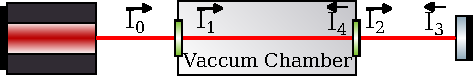
\includegraphics[width=0.95\textwidth]{graphics/windows-attenuation.pdf}
	\end{center}
	\caption{The effect of the Vaccum Chamber's windows' attenuation upon the LASER cooling intensities.}\label{fig:windows-attenuation}
\end{figure}

Since $\omega \equiv \Omega/\Gamma$ and $I \propto \Omega^2$, if we'd define\footnote{The experimentalist's most intuitive measurement is to measure $I_2/I_0$, but it should be equal $I_4/I_1$ assuming all windows are made of identical glass, and the intensity lost in the mirror is 0.} $\alpha \equiv I_4/I_1$, the actual force we are imposed to apply upon our ions is:

\begin{equation}
	\mathbf{F}(\mathbf{v}, \omega) - \mathbf{F}(-\mathbf{v}, \sqrt{\alpha}\omega)
\end{equation}

Causing a slight imperfect oddness (with respect to $\mathbf{v}$) of the force, depending on the windows attenuation parameter $\alpha$.

\subsubsection{Summery}

This is a good place to pause and list all the simulation parameters we collected from the theory above:

\begin{itemize}
	\item The LASER cooled ion. Choosing an ion and a cooling transition is effectively choosing $\lambda$, $\gamma$ and the mass $m$.\footnote{Cooling transitions and line-widths were taken from \cite{CoolingBeParameters,CoolingCaParameters1,CoolingCaParameters2,RansfordThesis,RadiumData}}. Current experimental efforts as well as all simulations presented focus on \ce{Yb^+}, but in principal this parameter is not hard-coded, and 
	\item The normalized LASER's intensity $\omega \equiv \Omega/\Gamma$.
	\item The normalized LASER's detuning $d \equiv \delta/\Gamma$.
	\item The spatial direction(s) of the LASER(s). This can be parameterized by a list of $(\theta, \phi)$ pairs - a pair per LASER, defining each LASER's $\hat{k}$ using a spherical coordinates transformation.
	% TODO: Consider whether adding this
	%\item Whether to use the approximated Taylor expression with only the 1st order term. This is not really a physical simulation parameter, but it was studied because I couldn't find simulations simulations in literature not using the approximation.
	\item The Vacuum chamber's windows' attenuation. Our experiment's attenuation is $\alpha = 0.7$, and most simulations use this value.\footnote{Besides figure ... which displays it's effect.}
	% TODO: \ref{fig:windows-attenuation-effect} in the results
\end{itemize}

Lastly, the relation of the Rabi frequency $\Omega$ to the actual LASER intensity\cite{CJFootOmega2I}, is worth mentioning\footnote{The software is capable of displaying $\omega$ dependence in the scale of the intensity $I$, but this behavior wasn't activated in the results presented.}:
% TODO: Make sure the above footnote is correct

\begin{equation}
	I = \frac{2\pi h c \Gamma}{3 \lambda^3} \cdot \left(\frac{\Omega}{\Gamma}\right)^2
\end{equation}

\subsection{Time Periods}

To fully define a simulation, one has to define a few more parameters. Two of which are related to the timeline and are referred to as cooling and stabilizing time. The cooling time period has trivial meaning and increasing it can be interesting but naturally the price is higher computing resources demands. The stabilization time is the time since $t=0$ up to the point where the LASER cooling force enters. For researching cooling parameters, and for most initial temperatures, there is no need for more then $5-7\mathrm{ms}$ of stabilizing time, just to let the thermodynamic instabilities of the initial conditions minimize. Figure \ref{TODO1} can serve as a good example in which the width of $T(t)$ before the LASER cooling starts decreases enough after $5 \mathrm{ms}$.

\label{TODO1}

Another usage for varying the stabilization time, is for measuring the eigenfrequencies of the trap, without cooling ($0$ cooling time), and all cooling parameters irrelevant.

\subsection{Time Dividing Finesse}

Another fairly technical parameter is the finesse of the time division. As further justified in subsection \ref{ssec:T_rf_type}, we want to always divide the simulation to an integer number of RF cycles. Since the RF frequency is also the highest frequency of the system, the natural thing to do is to divide each RF cycle to an integer number of steps, and this slightly arbitrary parameter is called the RF divisor. There is no theory that predicts an optimal RF divisor, and still this is a rather important technical detail:

One can perform many simulations with a certain RF divisor, and only in a specific simulation, in a specific advanced time, notice a certain ion has experienced a non-physically strong Coulomb force, causing it to fly way very far away, making the temperatures measurements noisy throughout the rest of the simulation, and hence essentially incorrect. With way too low RF divisors the temperatures measurements will be noisy and incorrect from the start. After a few months of optimizing this parameter, a value for the RF divisor was stabilized around $\sim 1500$. To further tighten the demand of the RF division's independence from potential numerical errors, a prime number was chosen.\cite{primesieve} More examples demonstrating effects of low RF divisors, and hence proving convergence for RF divisors $\sim 1500$, are available in section \ref{sec:init-conditions}.
% TODO: The above ref may need to be updated.

\subsection{Initial Conditions}

Lastly, the initial conditions were obtained using a random number generator with a specific seed. Each seed integer represents a reproducible set of initial conditions, given the algorithm distributing positions and velocities stays the same. To decouple the (small) effects of initial conditions upon the results, the same simulations but with different seeds were ran, and in most results displayed this dimension was averaged over.

% Put all the onenote's technical challenges related content here

\section{Output Result Types}

Naturally, the main result that interests us is the temperature. Which is essentially a common measure for the average kinetic energy, and in our case, since we use a VMI, it is a measure of the velocities' distribution's width. A physically related property of our ion clouds is the size, that can be measured per axis simply via a \texttt{std}. As for the temperatures, there are a few more ways to measure them, laid out below. 

\subsection{Temperature's Random Variables}

Under the approximated treatment of the Ion trap's potential as a perfect harmonic potential, and with the long range Coulomb potential neglected, one can treat the positions analogously, and hence almost identically to the velocities. This is done by multiplying each particle's position $x_i$ in the $i$'th axis, by $2\pi f_i x_i$, where $f_i$ is the secular frequency of the Ion trap in the $i$'th axis.\footnote{Although not implied by an existence of an additional index besides $i$, there is a different, non-trivial set of $f_i$ secular frequencies per particle species, as described in section \ref{ssec:params-trapping}.}
% TODO: Make sure the above ref is specific as possible

% TODO: Use labels per these temperatures related subsections, and \ref to them in the technical part of the thesis.
\subsection{Temperature's Probabilistic Methods}

Given $N$ particles, which were 'measured' during the computer simulation in a certain time, 2 arrays of shapes \texttt{(N,3)} are obtained for velocities and positions. The positions' array can be scaled by the proper secular frequencies as described above, and the question of how to compute a temperature given such an array has multiple legitimate answers. To layout all available answers we'll denote the random variable $u_i \in \{v_i, 2\pi f_i x_i\}$ for axis $i$. The $i$'th slice of length \texttt{N} from the above \texttt{(N,3)} shaped array is a distribution of the $u_i$ random variable.

One simple answer which is most intuitive in the context of VMI based measurements is to simply compute $m \mathrm{Var}(u_i)/K_\text{B}$, as derived from the Maxwell-Boltzmann distribution expression:

\begin{equation}
	f(\mathbf{u}) \mathrm{d}^{3}\mathbf{u} = \left[\frac{m}{2\pi k_{\text{B}}T}\right]^{3/2}\,\exp \left(-{\frac {m \mathbf{u}^2}{2K_\text{B} T}}\right) \mathrm{d}^{3}\mathbf{u}
\end{equation}

Another approach, is to integrate over a solid angle of $\mathbf{u}$ in the probabilistic model above, and write a speeds-like distribution function:

\begin{equation}
	f(|\mathbf{u}|) = \left[{\frac{m}{2\pi K_\text{B} T}}\right]^{3/2} 4\pi |\mathbf{u}|^{2}\exp\left(-{\frac{m |\mathbf{u}|^{2}}{2k_{\text{B}}T}}\right)
\end{equation}

Which has a variance equal to $K_\text{B} T/m \cdot (3 - 8/\pi)$, and a squared mean equal to $K_\text{B} T/m \cdot 8/\pi$, thus providing 2 more methods to calculate a temperature given a \texttt{(N,3)} shaped array of either positions or velocities.

\subsection{Temperature Under the Secular Approximation}\label{ssec:T_rf_type}

In addition to the velocities and/or positions choice of random variable(s), and in addition to the above probabilistic model approaches, one has to decide how to imitate the secular approximation computationally. The physical justification for doing it, is the fact that in a crystal phase (which we aim achieving), the movement of the ions is strongly coupled to the RF field which we have direct control over. Essentially the model states that the collective movement due to the RF field is predictable and so well defined, that it is not a random variable.

Experimentally speaking, we are capable of measuring positions and velocities always at the beginning/end of each RF cycle, and hence always use an integer number of RF cycles. This is the simplest and probably the only way of implementing a secular approximation experimentally, and it should work best for ions that have formed a crystal. In the following, we'll describe what other techniques are available to a computer simulation that might help achieve time dependent, secularly approximated temperature measurements.\footnote{There's also a technical motivation to imitate some kind of secular approximation when measuring temperatures, and that is reducing the amount of disk writes required when simulating $\sim 3,000$ RF cycles divided to $\sim 1500$ time steps. Reducing the amount of disk writes not only reduces disk usage of simulation result files, but also speeds up the total time required for simulating.}

% TODO: Cite stuff from zothero regarding RF averaging..
Besides sampling the velocities and positions in the beginning of each RF cycle, many simulations based research found in literature average over an RF period each particle's per-axis velocity, and then construct a temperature. You might hope that the same can be done for $2\pi f_i x_i$, but apparently, even for ion clouds initiated in a thermal gas phase equilibrium in temperatures as low as $5\mathrm{K}$, each particle reaches many spatial areas of the trap, and it's RF averaged position produce (incorrect) temperatures in the $\mathrm{\mu K}$ regime! This proves that this approach is not accurate also for the velocities, at least for gas like phases, as it suggests that ions go through a big part of the phase-space. Never the less, I decided to do save the RF averaged velocities (but not the positions) to the disk during simulations, and the software displaying the simulation results provides the option to use this data.

Another interesting RF cycles related option, is to sample the velocities and positions in the middle of each RF cycle - where the kinetic energy induces by the RF field should be at it's peak. The difference from the energies in the beginning of the RF cycles may help extract the RF motion energy. This data was also saved for both positions and velocities, for consistency.

\subsection{Temperatures Options Summary}\label{ssec:T-options-summery}

The above temperatures related options are modeled in software as 3 dimensions with the names and symbolic optional values as defined in table \ref{tbl:T_methods}

\begin{table}
\begin{tabular}{l||l|l|l|l|l}
Dimension   & \multicolumn{5}{c}{Optional values}\\
\hline\hline
% TODO: Maybe T_coord is not a good name?
 \texttt{T\_coord}   & $\vec{v}$                                    & \multicolumn{2}{l}{$\overrightarrow{\omega x}$} \\
\hline
\texttt{T\_rf\_type} & $\left\langle\circlearrowright\right\rangle$ & $\mathrm{min}\left(\circlearrowright\right)$ & \multicolumn{2}{l}{$\mathrm{max}\left(\circlearrowright\right)$} \\
\hline
\texttt{T\_method}  & $\mathrm{Ave}\left(|u|\right)^2(\pi/8)$      & $\mathrm{Var}\left(|u|\right)/(3 - 8/\pi)$   & $\mathrm{Var}\left(u_x\right)$               & $\mathrm{Var}\left(u_y\right)$ & $\mathrm{Var}\left(u_z\right)$ \\
\hline
\end{tabular}
\caption{Ways to measure temperatures, obtained from a generalized maxwell-Boltzmann model}
\label{tbl:T_methods}
\end{table}

Where $\circlearrowright$ marks an RF cycle, and $\left\langle\circlearrowright\right\rangle$ marks an average over RF cycle. The functions $\mathrm{Ave}$ and $\mathrm{Var}$ operate upon a 1 dimensional array of length $N$ - the number of particles sampled.

Lastly, we can select specific, multiple temperature values and average over the different methods, coordinates and RF methods. A common example is to take the positions and velocities sampled in the beginning of each RF cycle ($\mathrm{min}\left(\circlearrowright\right)$), and calculate the temperature according to all the \texttt{T\_method}s. Whatever specific \texttt{T\_coord}s / \texttt{T\_rf\_type}s / \texttt{T\_method}s were chosen, the code analyzing and displaying the simulation results averages over these dimensions while keeping the time dependence of course.\footnote{Technically, the temperatures obtained from the RF averaged ($\left\langle\circlearrowright\right\rangle$) positions ($\overrightarrow{\omega x}$) are considered \texttt{NaN} and hence ignored.}

\subsection{Further Summarizing Analyzes}

Up until now we discussed time dependent properties of our ion clouds - the per spatial axis size and the various temperatures. We can also summarize these results to obtain various measures of how fast did we cool our ions, and how much smaller did the cloud get due to the LASER cooling etc. This is termed both in the code and here as summarized results.

The simplest summarized result type is the temperature/size after the cooling process, which is defined (slightly arbitrarily) as the average temperature/size of the ion cloud in the last 1/4 of the time before cooling or before the end. The first \textit{part} is referred to as \textit{stabilizing part} and the later \textit{cooling part}. The standard deviation of the temperature/size in each such \textit{part} defines the uncertainty for each such summarized measurement. The size measurement, both in the time dependent form and in the summarized form depends on the spatial axis (x,y,z), and the temperatures, in either the summarized or time dependent form, depend on the 3 dimensions described in subsection \ref{ssec:T-options-summery}.

Another summarized measurement is the cooling frequency, defined (for simplicity, only for temperatures) as follows: Given a $T(t)$ defined using any of the parameters of subsection \ref{ssec:T-options-summery}, we take $Log(T(t)/\mathrm{kelvin})$, and apply a continuous piecewise linear fit\cite{pwlf}, with 2 segments. This gives 2 cooling frequencies in the units of $\mathrm{kHz}$ that depend on a dimension referred to as \texttt{regime}. This design choice stems from the observation that in many simulations most of the ion cloud is cooled quickly and efficiently whereas afterwards the rest of the cooling happens in a mixed thermodynamic phase of an ion crystal (massive and highly charged) with a gas of ions surrounding it. The initial, faster and more efficient part of the cooling process corresponds to the 1st segment of exponential temperature decay, and the rest of the cooling is significantly slower, and hence invite defining a 2nd segment of cooling.

Lastly, only for verifying the frequencies expected from the Mathieu equations of the ion trap, as explained in subsection \ref{ssec:params-trapping}, we define the following analysis referred to as the \textit{cloud's frequencies}: Given the time dependent positions of all ions, we average over the ions to get the cloud's center position (still time and spatial axis dependent). With it, we can take the Fourier transform and get the dominant frequency via \texttt{scipy.signal.find\_peaks}\cite{scipy}, or simply via \texttt{numpy.argmax}\cite{numpy}. If the collective movement is very harmonic (due to e.g collective offset in which the ion cloud was intentionally placed at $t=0$), a fit for a $\cos(2\pi f x_i + \phi)$ can be attempted, and the fit's frequency is the dominant frequency of movement. The time range of the simulation dictates the uncertainty in the dominant frequency obtained via a Fourier transform, and the dominant frequency of the fit produces uncertainties via the covariance matrix returned by \texttt{scipy.optimize.curve\_fit}.


%
% and then cover:
% - The methods used in the research
% - The research results
% - Discussion and conclusions from the results
%
% but not necessarily with a specific chapter for each of them.
%
% Then you have your main chapters (although these might still
% include an initial chapter on technical preliminaries, experimental
% system setup, and/or a final chapter with summary, discussion and further
% research direction or questions)

\chapter{Computational Challenges prior to Simulating}

\section{Converting Secular Frequencies to Electric Fields}\label{sec:comp/freqs2aq}

% TODO: Cite more places that solve the Mathieu equation from a geometry of electrodes.
Most solutions of the Mathieu equation in the context of ion trapping start from a certain physical design of electrodes, that (often loosely\cite{AkermanThesis}) is justifying a certain parametrisation for 3 dimensional Mathieu equations. Our only geometry based assumption is that $q_z = 0$, as explained in subsection \ref{ssec:params-trapping}. The following subsections will dive deeper into details of the Mathieu Equation solution, and present a few insights relevant to sympathetic cooling. 

\subsection{Dimensionless Mathieu Equation Solving}

For the sake of completeness, I'll quickly explain how to solve the 1 dimensional Mathieu equation in a numerically practical way. My implemented parametrisation aligns with most parametrisations found in literature:

\begin{equation}
	(a + 2 q \cos(2 \tau)) x = \ddot{x}
	\label{eq:bare-mathieu}
\end{equation}

Substituting a solution of the form:\footnote{Note that $\beta \ne \omega_{rf}/\omega_\mathrm{sec}$ but rather: $\omega_\mathrm{sec} = \beta \omega_{rf}/2$}

% TODO: Write this equation
$$x(\tau) = \sum_{-\infty}^\infty $$

Yields the set of equations presented in \ref{eq:gamma_n-relation} between the coefficients $\{\gamma_n\}_{-\infty}^\infty$. The main point important to understand, is that we need to find a non-trivial solution, meaning a set $\gamma_n$ coefficients that not all are $0$. The best way to view the equations of all coefficients is via a matrix:

\begin{equation}
% Generated by ChatGPT using the Python code :)
\begin{bmatrix}
\ddots & \ddots & \ddots & & & & \vdots & \vdots & \\
\ddots & -D_{-N} & 1 & 0 & \cdots & 0 & 0 & 0 & \cdots \\
\ddots & 1 & \cdots & \cdots & \cdots & \cdots & \cdots & 0 & \cdots \\
& 0 & \cdots & -D_{-1} & 1 & 0 & \cdots & 0 & \\
& \vdots & \cdots & 1 & -D_0 & 1 & \cdots & \vdots & \\
& 0 & \cdots & 0 & 1 & -D_{1} & \cdots & 0 & \\
\cdots & 0 & \cdots & \cdots & \cdots & \cdots & \cdots & 1 & \ddots \\
\cdots & 0 & 0 & \cdots & 0 & 1 & -D_{N} & \ddots & \ddots \\
& \vdots & \vdots & & & \ddots & \ddots & \ddots & \ddots \\
\end{bmatrix}
\begin{bmatrix}
\vdots \\
\gamma_{-N} \\
\vdots \\
\gamma_{-1} \\
\gamma_0 \\
\gamma_{1} \\
\vdots \\
\gamma_{N} \\
\vdots
\end{bmatrix}
\overset{!}{=}
\begin{bmatrix}
\vdots \\
0 \\
\vdots \\
0 \\
0 \\
0 \\
\vdots \\
0 \\
\vdots
\end{bmatrix}
\end{equation}

Where similarly to \ref{eq:gamma_n-relation}:

$$D_n = \frac{a - \left(\beta + n\right)^2}{q}$$

One can easily see that $D_n$ increases $\sim n^2$, which promises the target $\beta$ solution might converge if a finite matrix will be used. To require a non-trivial solution, we simply require the matrix to have a $0$ determinant, thus supplying us an equation for $\beta$ that can be solved easily numerically, for matrix size $2N+1$. Inserting the $\beta$ into the matrix, and inspecting the kernel of it, will give us the $\gamma_n$ coefficients of the solution, and we'd be able to easily verify they indeed decrease with $|n|$, and are most dominant for $n=0$.

The verification of this solution was implemented in a Matplotlib\cite{Matplotlib} based interactive plot, presented in figures \ref{fig:pure-mathieu-coefficients} \& \ref{fig:pure-mathieu-fft}.

\begin{figure}
	\begin{center}
		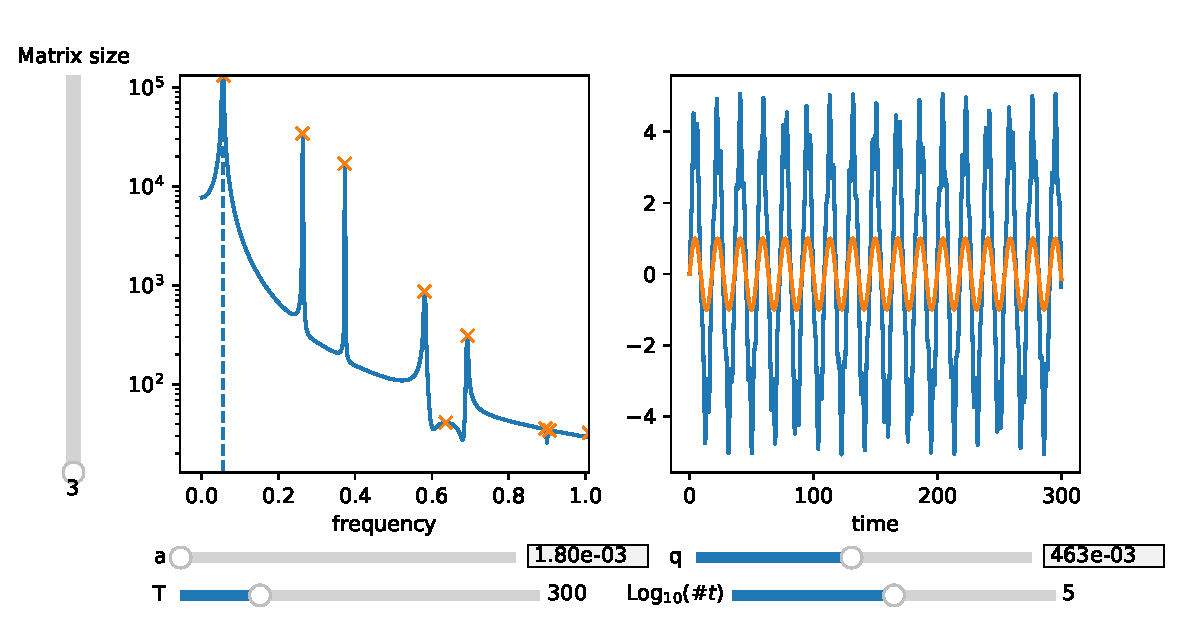
\includegraphics[width=0.95\textwidth]{graphics/pure-mathieu-fft.pdf}
	\end{center}
	\caption{Matplotlib interactive plot presenting the 1 dimensional solution of the Mathieu equation, with a spectrum analysis demonstrating the correct matrix based solution of $\beta$. The orange sinusoidal line in the right axes is a simple cosine line with the right phase and the calculated $\beta$ as a frequency. The $T$ and $\mathrm{Log}_{10}(\#t)$ sliders control the total time duration of the numerical ODE solution and the time spacing finesse, respectively.}
	\label{fig:pure-mathieu-fft}
\end{figure}

\begin{figure}
	\begin{center}
		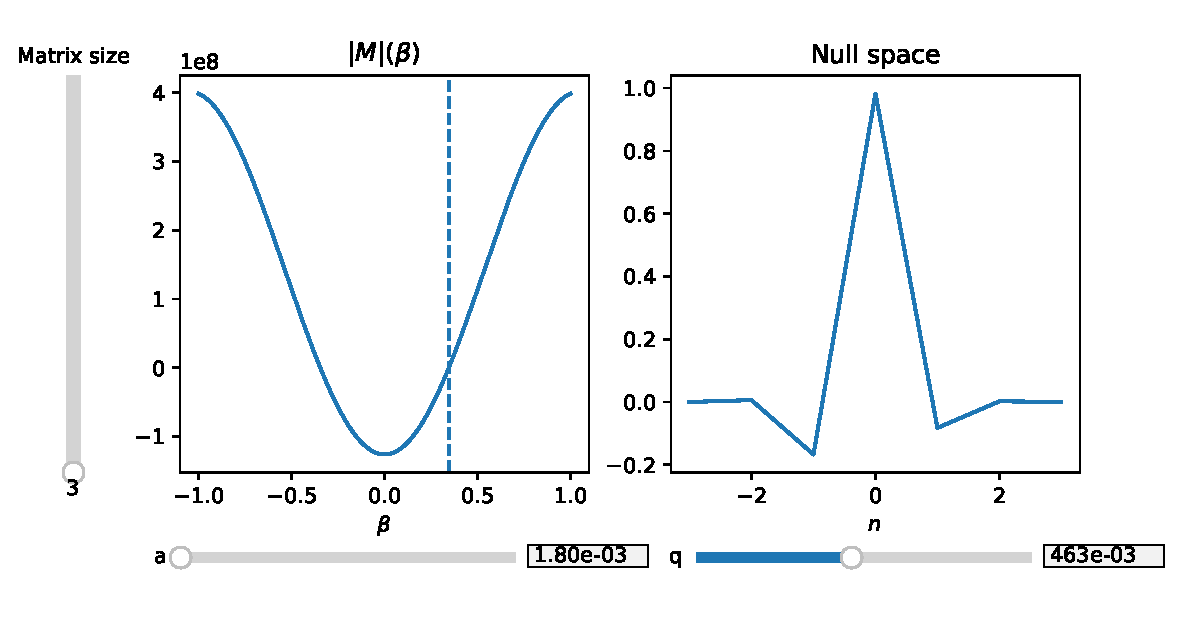
\includegraphics[width=0.95\textwidth]{graphics/pure-mathieu-kernel.pdf}
	\end{center}
	\caption{Matplotlib interactive plot demonstrating the fast decay of the Mathieu equation's solution's $\gamma_n$ (normalized) coefficients, as $|n|$ increases. The dashed $\beta$ line represents the $\beta$ which zeros the matrix determinant.}
	\label{fig:pure-mathieu-coefficients}
\end{figure}

Interactive plot \ref{fig:pure-mathieu-fft} can be also useful for inspecting the roughness of the motion as a function of $a$ and $q$. As expected, a high $q$ and a lower $a$ produce more 'RF-noisy' motion near the peaks of the oscillatory, secular motion. Also, satisfyingly, there's barely any difference in the $\beta$ accuracy as $N$ is increased, even starting from $N=3$. Hence this parameter was practically hard-coded in all the simulations etc. to $N=7$.

% TODO: Cite this
Most Mathieu stability diagrams found in literature, assume that geometry dictates $a_x = a_y$, and like us, that $q_z = 0$. Thanks to equation \ref{eq:laplace}, this suggests that one can plot a single Mathieu stability diagram for a 3 dimensional trap using a single Mathieu stability diagram for $(a_r,q_r)$ where $a_r \equiv a_x = a_y = -a_z/2$ and $q_r = q_x = -q_y$ as axes. I find these stability diagrams confusing, as they need to also take care of correctly mirroring $q_x = -q_y$ to satisfy stability in both $x$ \& $y$ spatial dimensions (where the $z$ axis is trivially stable). Figure \ref{fig:mathieu-stability} presents a much simpler alternative to show the stability of a 3 dimensional trap, without even imposing cylindrical symmetry which shouldn't be physically unimplementable.

\begin{figure}
	\begin{center}
		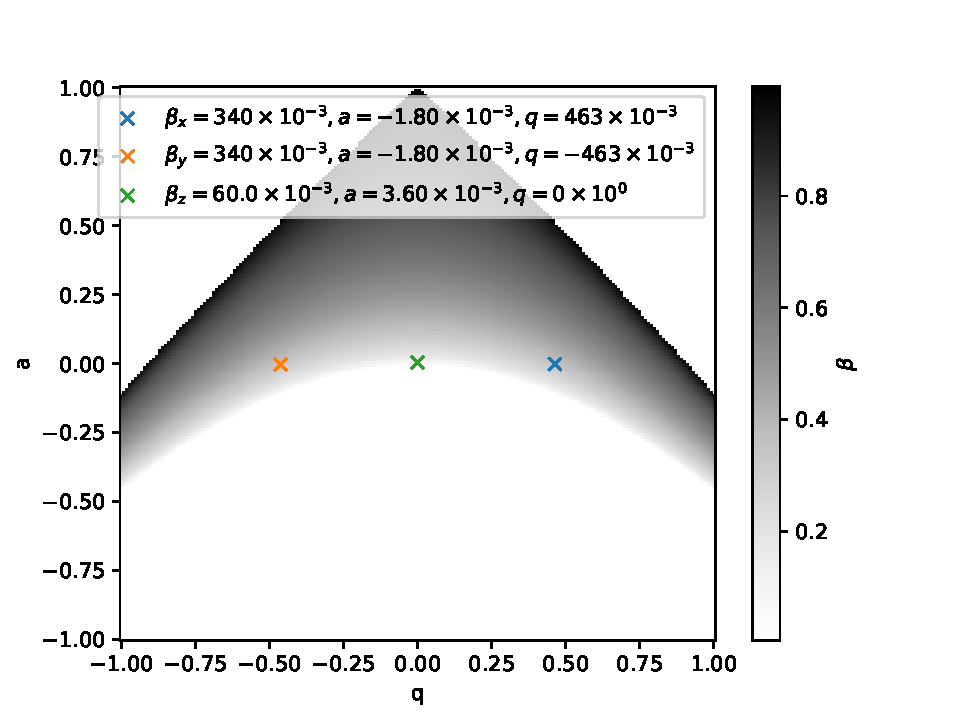
\includegraphics[width=0.86\textwidth]{graphics/pure-mathieu-stability.pdf}
	\end{center}
	\caption{Mathieu Stability diagram, with shades of gray marking the magnitude of $\beta$. The $\times$ signs are specific $\beta$ values, that were used in many simulations of this work - $\beta$s corresponding to secular frequencies $(8.5, 8.5, 1.5)\mathrm{kHz}$, with $f_{rf} = 50\mathrm{kHz}$.}
	\label{fig:mathieu-stability}
\end{figure}

\subsection{A Non-Trivial Secular Frequency Mass Dependence}\label{ssec:non-trivial-mass-dep}

In my literature I have seen no authors discuss the secular frequency related implications encountered when 2 different masses are trapped in the same Ion trap. This detail is naturally of interest to us as we are interested in sympathetic cooling. Let's discuss this question in 1 spatial dimension: Given a $(a,q)$ pair producing a dimensionless secular frequency $\beta_0$ for mass $m_{cooler}$, what would be the secular frequency experienced by a mass $m_{target}$ experiencing the same forces? In a pure harmonic oscillator, the same $k = m_{cooler} \omega_{\mathrm{sec(cooler)}}^2 = m_{cooler} (\beta_0 \omega_{rf}/2)^2$ is applied to any mass, and we get a secular frequency for $m_{target}$ of:

\begin{equation}
	\omega_\mathrm{sec(target)} = \omega_\mathrm{sec(cooler)}\sqrt{\frac{m_{cooler}}{m_{target}}} 
	\label{eq:mathieu-naive-sec-freq}
\end{equation}

Is that true in a Mathieu trap? The process of generating a dimensionless $(a,q)$ from the original equation of motion (equation \ref{eq:mathieu-source}) involves dividing the equation by the mass, meaning that $(a,q)\propto 1/m_{cooler}$. Hence the real secular frequency of $m_{target}$ can be obtained by calculating $\beta_{target}$ given the pair:

$$(a,q)\cdot \frac{m_{cooler}}{m_{target}}$$

The dependence of $\beta_{target}$ as a function of the mass ratio is depicted in figure \ref{fig:mathieu-mass-dep}. This insight invites defining 2 decoupled, boolean parameters for the simulation, named \texttt{micromotion} \& \texttt{naive\_freqs}. Table \ref{tbl:naive_freqs-micromotion} is a truth table explaining what trapping forces are applied in each combination of these parameters. A separate definition of these parameters is laid out afterwards for completeness.
% TODO: Make sure this 'afterwards' is correct - depends upon the final state of the document

\begin{figure}
	\begin{center}
		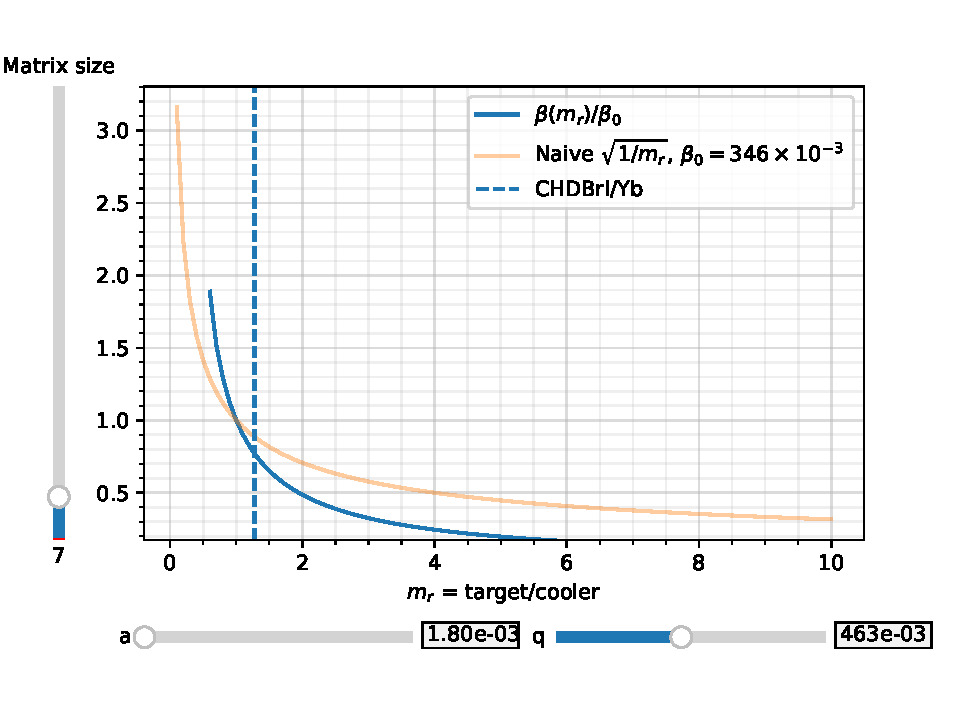
\includegraphics[width=0.86\textwidth]{graphics/mathieu-mass-dep.pdf}
	\end{center}
	\caption{A Matplotlib interactive plot showing the non-trivial dependence of the secular frequencies of a 'target' mass (represented in blue), given a Mathieu trap with $(a,q)$ that define a certain secular frequency for a 'cooler' mass, termed $\beta_0$. The $(a,q)$ values used here, implement the $x$-axis Mathieu force that was used in the simulations that produced the summarized results in figure \ref{fig:LAMMPS_summarized_naive_freqs-micromotion}, which also shows the possible secular frequencies' absolute values in $\mathrm{kHz}$.}
	\label{fig:mathieu-mass-dep}
\end{figure}

\begin{table}[h]
\centering
\begin{tabularx}{\textwidth}{cccX}
\toprule
\texttt{mm} & $\sqrt{m_r}$ & \textbf{Physical} & \textbf{Description} \\
\midrule
$\checkmark$ & $\times$ & $\checkmark$ & A single electric field exhibiting 3 dimensional Mathieu equations - The only physically possible kind of trap, with non-trivial secular frequencies as presented in figure~\ref{fig:mathieu-mass-dep}. \\
\midrule
$\times$ & $\checkmark$ & $\times$ & A single \(k \mathbf{x}\)-like force is acting upon all ions — implementing the naive frequencies you'd expect from a perfect Harmonic oscillator. \\
\midrule
$\checkmark$ & $\checkmark$ & $\times$ & Two different Mathieu forces are applied to each mass, such that the naive frequencies related by $\sqrt{m_r} \equiv \sqrt{m_{cooler}/m_{target}}$ are experienced by the two ion species. \\
\midrule
$\times$ & $\times$ & $\times$ & Two different \(k \mathbf{x}\)-like forces are applied to each mass, such that the non-naive frequencies are experienced by the two ion species. \\
\bottomrule
\end{tabularx}
\caption{Truth table for \texttt{micromotion} (\texttt{mm}) and \texttt{naive\_freqs} ($\sqrt{m_r}$) combinations and their physical validity.}
\label{tbl:naive_freqs-micromotion}
\end{table}

\subsubsection*{\texttt{naive\_freqs} ($\sqrt{m_r}$)}

Controls whether the secular frequencies experienced by the target \ce{CHDBrI^+} ion are defined using the 'naive' $\sqrt{m_r}$ relation. Turning this option on naturally implements a trap that is not physically implementable.

\subsubsection*{\texttt{micromotion} (\texttt{mm})}

Controls whether the secular frequencies experienced by both ion species are implemented using a Mathieu like force like in equation \ref{eq:mathieu-source}, or using a perfect harmonic trap force like $k \mathbf{x}$. A perfectly harmonic trap is of course not implementable.

\subsection{LAMMPS Verification of Mathieu Understanding}

Now that we have gained confidence in our Mathieu solving capabilities, Let's demonstrate that indeed the reversely solved Mathieu equations presented in subsection \ref{ssec:params-trapping} indeed produces $(a_i, q_i)$ pairs with the requested secular frequencies. Figure \ref{fig:LAMMPS_summarized_naive_freqs-micromotion} demonstrates that decoupling the \texttt{micromotion} and \texttt{naive\_freqs} parameters was done successfully.

\begin{figure}
	\begin{center}
		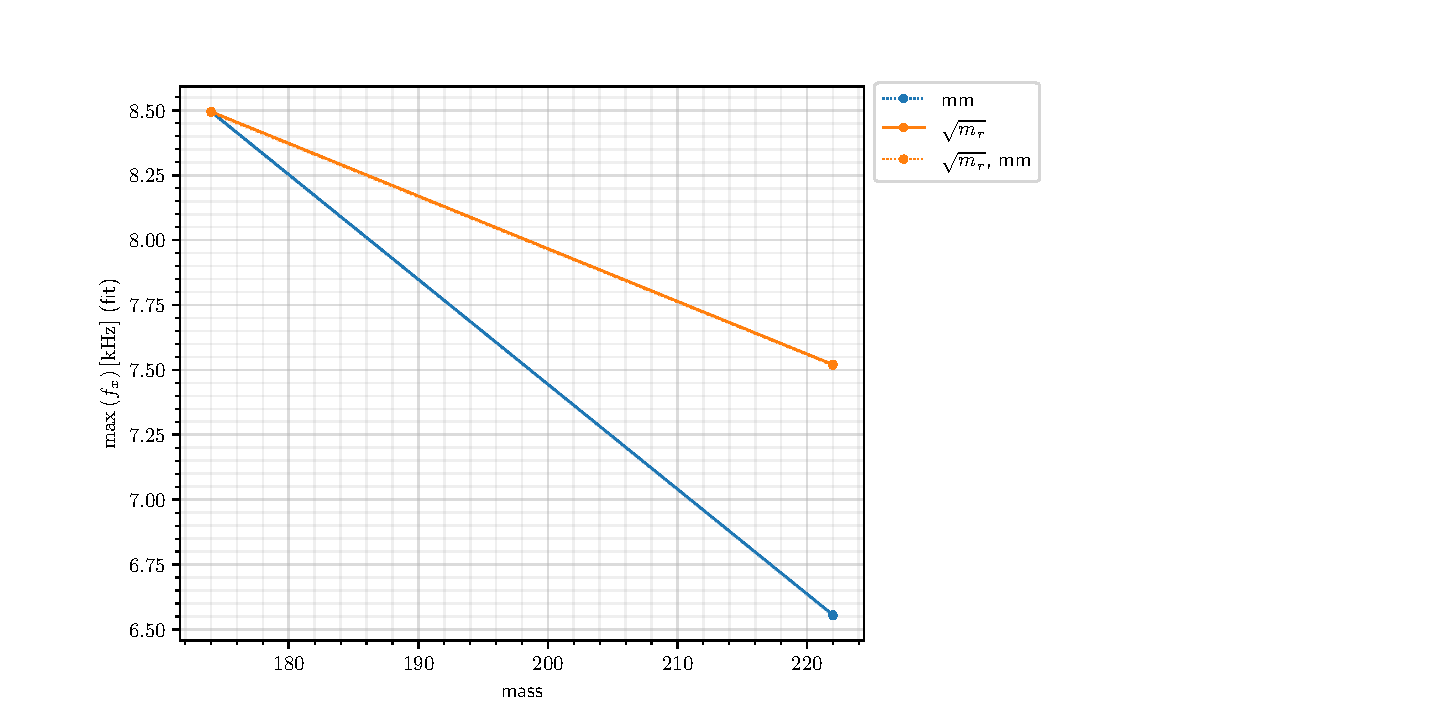
\includegraphics[width=1.2\textwidth]{graphics/micromotion_and_sqrt_freqs_effect.pdf}
	\end{center}
	\caption{The collective $x$-axis movement's frequencies of a 2-species-mixed ion cloud, positioned in a spatial offset from the origin at $t=0$. Dashed v.s solid line-style represents whether \texttt{micromotion} was enabled, and the \texttt{naive\_freqs} parameter is represented in color. The color-varied behavior demonstrates the non-negligible difference between the naive, $\sqrt{m_r}$-based calculation and the real frequencies that are experienced in a real ion trap. Looking closely, you should observe that the dashed lines are right on top of the solid lines - proving that indeed the simulation code was capable of putting the correct forces no matter whether \texttt{micromotion} was enabled or not. The only physically implementable line is the dashed \texttt{mm} labeled line. This figure was generated via fitting the cloud's center to a cosine, and via extracting the optimized frequency. Almost identical results can be obtained via using \texttt{numpy.fft.fft}\cite{numpy}.}
	\label{fig:LAMMPS_summarized_naive_freqs-micromotion}
\end{figure}

\section{Coulomb Energy Effect on Temperature}\label{sec:comp/coulomb}

We wish to study sympathetic cooling starting from a thermodynamically stable state. This helps reduce the random effects of thermodynamic instabilities, which can be computationally expensive to ignore, although in experiment, these instabilities might not affect much the cooling. This raises a few important questions: How significant is the Coulomb potential energy in the Boltzmann ensemble? Should it be considered when initiating the positions and velocities of the ions?

Under the secular approximation, and when ignoring the Coulomb potential, the Maxwell-Boltzmann partition function dictates the probability of finding an ion in a position $\mathbf{x}$ to be:

\begin{equation}
	\prod_{i=1}^3 \sqrt{\frac{k_i}{2\pi K_\text{B} T}} \exp\left(\frac{-k_i x_i^2}{2 K_\text{B} T}\right)
	\label{eq:position-probability}
\end{equation}

Where $k_i$ is the spring-like coefficients of the harmonic trap. This distributions couples naturally density and temperature. We are interested in measuring the Coulomb energy per particle (denoted as $E_c/N$) as a function of the parameters of the distribution function above. Since the real temperature is affected by the Coulomb energy, we will not use the symbol $T$ in the following usages of expression \ref{eq:position-probability}, but rather we'll use $\tau$. The parameters that can affect $E_c/N$ are: $\{k_i\}$, $\tau$, and most importantly the number of ions $N$.

The relation of $E_c/N$ to it's parameters is not analytical, yet we still expect a smooth behavior if we'd average over enough randomness. In figure \ref{fig:coulomb_energy} we can see that (expectedly), dense and cold ion clouds produce a higher Coulomb energy, that even exceeds $\tau$.\footnote{Figure \ref{fig:coulomb_energy_normalized} to appendix shows the same results normalized to $\tau$.}

\begin{figure}
	\begin{center}
		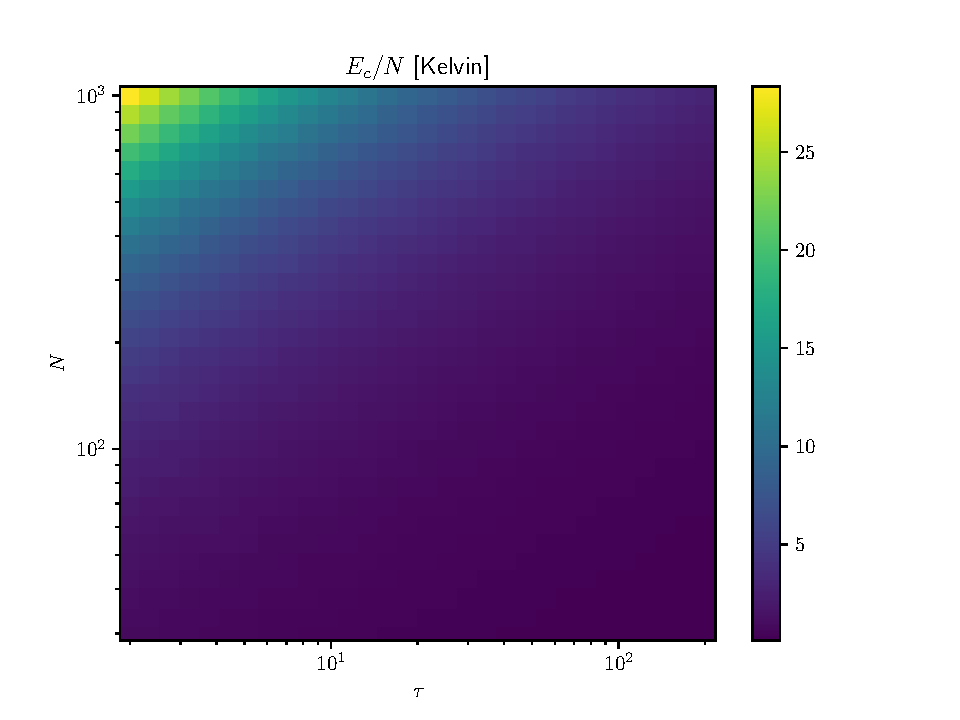
\includegraphics[width=0.95\textwidth]{graphics/coulomb_energy_example@coulomb_energy.pdf}
	\end{center}
	\caption{Example dependence of $E_c/N$ to $N$ and $\tau$ for a trap of \ce{Yb^+} with secular frequencies of $(8.5, 8.5, 1.5) \mathrm{kHz}$, in the range of $\tau\in[2, 200]\mathrm{K}$.}\label{fig:coulomb_energy}
\end{figure}

To produce this color-mesh, we distributed the ions in space multiple times per $(\tau,N)$ point, until the relative standard deviation of all $E_c/N$ results in that point was lower then $0.12$ (arbitrary number), with a minimum of 5 distributions (also termed 'iterations'). Statistical results of figure \ref{fig:coulomb_energy} is depicted in figures \ref{fig:coulomb_energy_std} and \ref{fig:coulomb_energy_iterations}.

Naturally, the value of the highest Coulomb energy found escalates with the trap's tightness, as can be seen in figure \ref{fig:coulomb_energy_f_z}.

\begin{figure}
	\begin{center}
		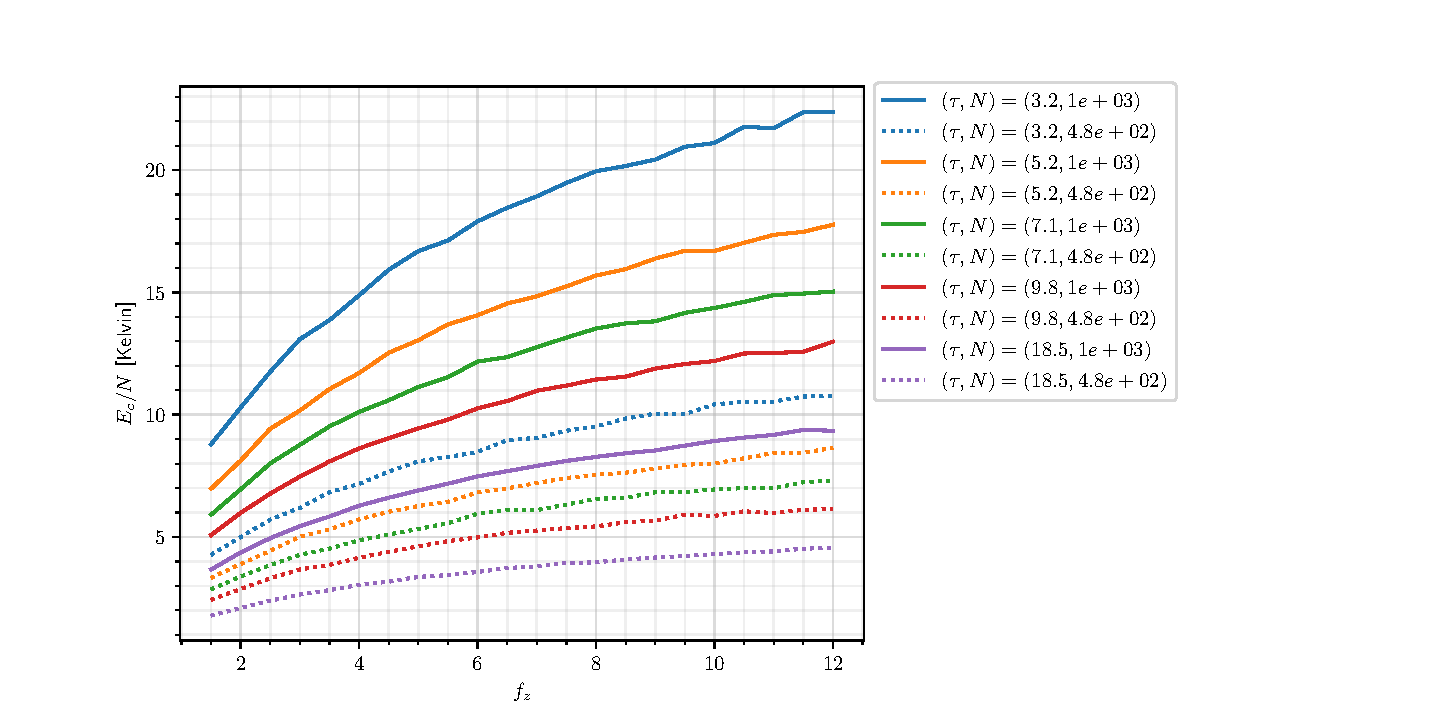
\includegraphics[width=1.2\textwidth]{graphics/coulomb_energy_f_z.pdf}
	\end{center}
	\caption{The dependence of $E_c/N$ upon the z secular frequency, for a few specific $(\tau,N)$ pairs, and $f_x = f_y = 8.5\mathrm{kHz}$.}\label{fig:coulomb_energy_f_z}
\end{figure}

To \textbf{summarize}, the Coulomb energy is not negligible for dense \& cold distributions. Our ability to initiate a distribution of ions in a thermodynamically stable set of positions is limited by the effects of strong Coulomb energy, and by the tightness of our trap. To avoid too strong Coulomb energy effects, we thereby avoid distributing ions in $T < 5\mathrm{K}$.\footnote{During the research period I tried to construct an algorithm that would get a real temperature $T \ne \tau$, $N$ and a set of secular frequencies, and compute a $\tau$ with which the system will be more thermodynamically stable initially. When this algorithm was used for a single ion species it was slightly effective. However when 2 ion species were used, (with different masses and different $\{k_i\}$ - see section \ref{sec:comp/freqs2aq}), accommodating the algorithm for that case has proved to be too complex, and too slow.} More importantly, we expect time dependent temperature measurements to be offset from the initial temperature $T_i$ on the order of magnitude of the Coulomb energy. Since we also wish to start cooling when the system is thermodynamically stable, the Coulomb energy offset requires us to wait for a few $\mathrm{ms}$, before beginning cooling, as can also be seen from the oscillations in figure. % TODO: \ref{fig:} from results

\section{RF division Finesse, Stability \& Convergence}\label{sec:comp/convergence}

% TODO: Explain how RF division is critical.

\chapter{Cooling Simulations}\label{cooling-simulations}

\section{LASER cooling parameters}\label{laser-cooling-parameters}

\subsection{\texorpdfstring{Intensity (\(\Omega/\Gamma\)) \& Vacuum
Chamber Windows
Attenuation}{Intensity (\textbackslash Omega/\textbackslash Gamma) \& Vacuum Chamber Windows Attenuation}}\label{intensity-omegagamma-vacuum-chamber-windows-attenuation}

\subsection{\texorpdfstring{Detuning (\(\delta/\Gamma\))}{Detuning (\textbackslash delta/\textbackslash Gamma)}}\label{detuning-deltagamma}

\section{LASER Cooling Intrusion Angle(s) \& Trap Geometry}\label{laser-cooling-intrusion-angles-trap-geometry}

\section{\ce{CHDBrI+} Concentration \& Total \#Ions Dependence}\label{chdbri-concentration-total-ions-dependence}


\chapter{Conclusion and open questions}
\label{chap:conclusion}

This kind of chapter can include may different things (or only some of them):
\begin{itemize}
\item Discussion of results
\item Conclusions from the results or from the process in general
\item Open questions for future research, resulting from the research performed or from the results obtained
\end{itemize}

But not things like the bibliography or other back matter which is generated outside of this chapter.

\section{Some conclusion}

Here is what I conclude.

\section{Some open questions}

%
% Add any appendices here; they must come _before_ the bibliography
%
\appendix
\chapter{More Coulomb Energies Dependence Figures}\label{chap:coulomb}

\begin{figure}[h]
	\begin{center}
		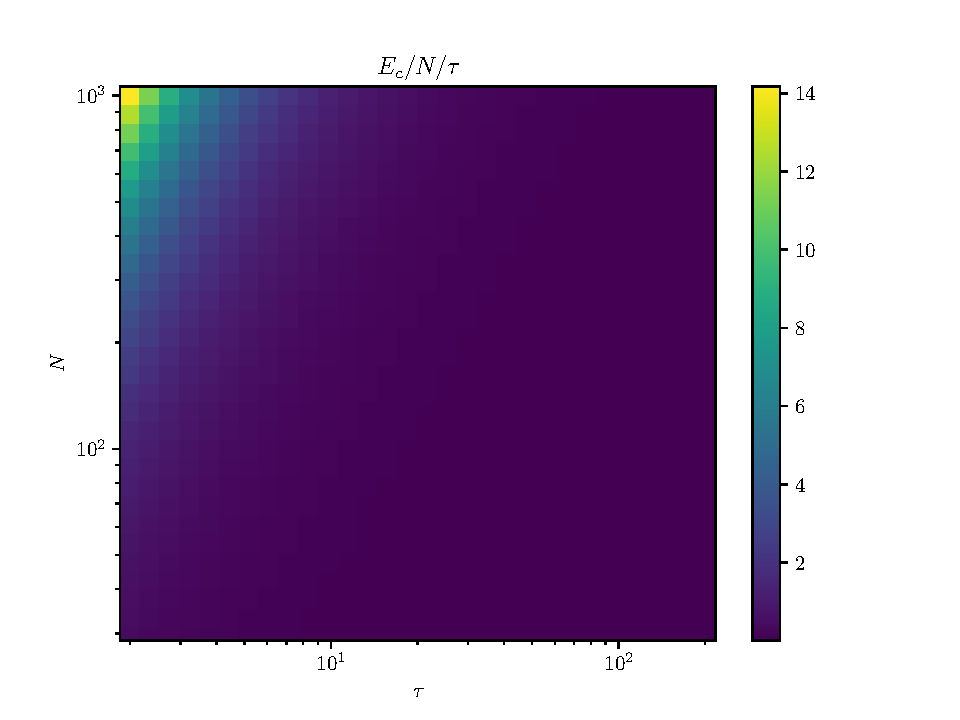
\includegraphics[width=0.9\textwidth]{graphics/coulomb_energy_example@relative_coulomb_energy.pdf}
	\end{center}
	\caption{Same as figure~\ref{fig:coulomb_energy}, but with a normalization to $\tau$. Added here to show how $E_c/N$ can exceed $\tau$ for some values of $(\tau,N)$.}
	\label{fig:coulomb_energy_normalized}
\end{figure}

\begin{figure}
	\begin{center}
		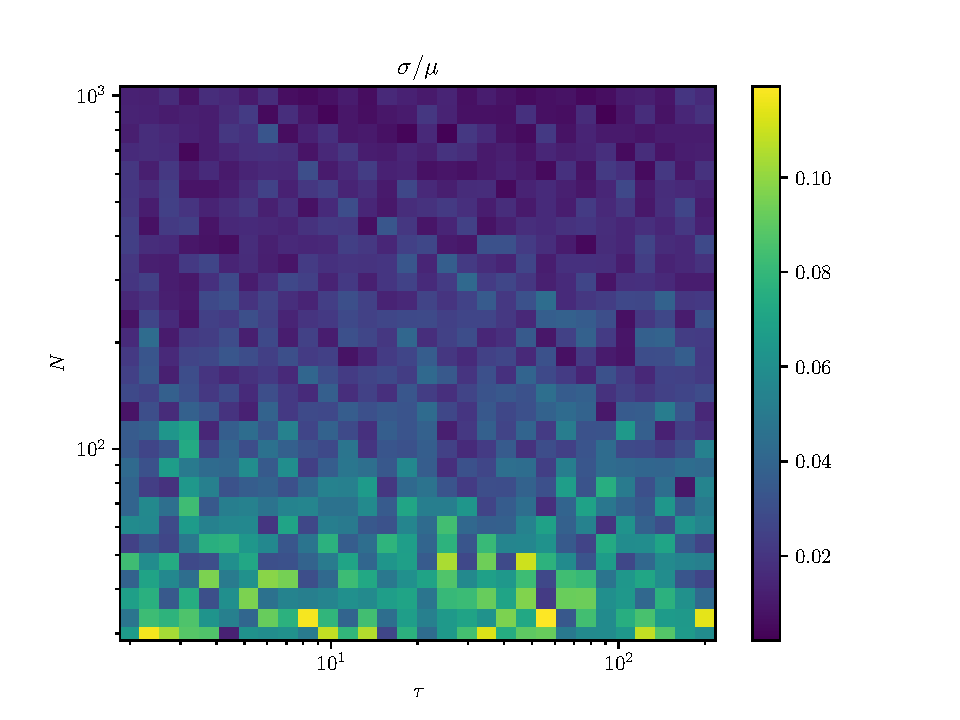
\includegraphics[width=0.85\textwidth]{graphics/coulomb_energy_example@relative_std.pdf}
	\end{center}
	\caption{The relative standard deviation received when generating figure~\ref{fig:coulomb_energy}. Naturally, in low $N$ (low-densities), the randomness is larger.}
	\label{fig:coulomb_energy_std}
\end{figure}

\begin{figure}
	\begin{center}
		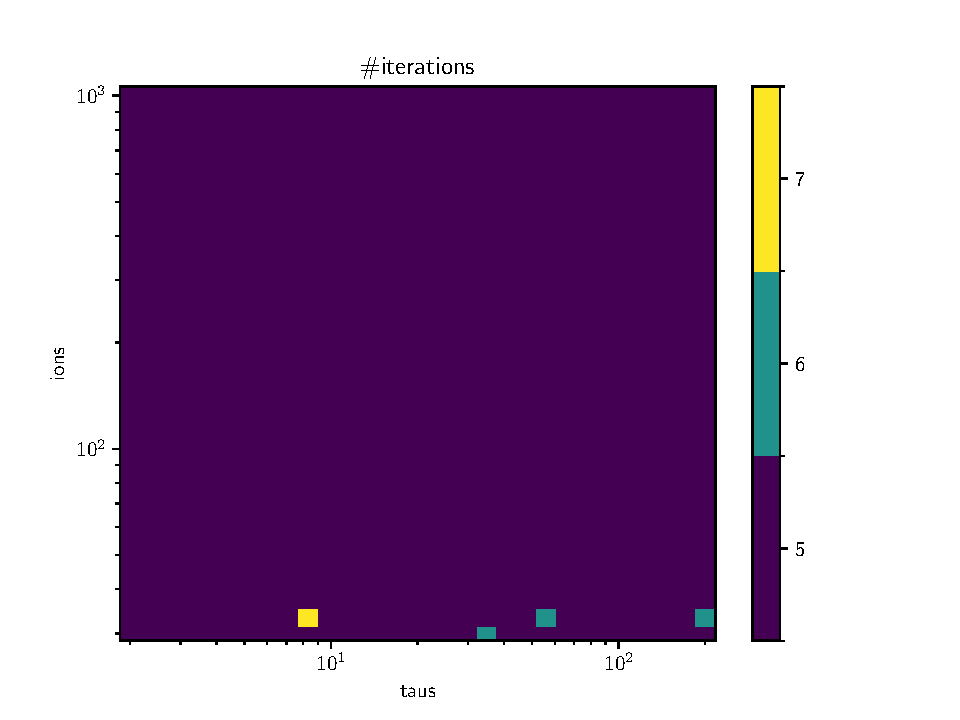
\includegraphics[width=0.85\textwidth]{graphics/coulomb_energy_example@iterations.pdf}
	\end{center}
	\caption{The number of iterations that had to be performed to generate each point in figures \ref{fig:coulomb_energy}. Almost always 5 random number generations is enough to reach a relative standard deviation smaller then $0.12$, however sometimes a few more iterations are needed, naturally for small $N$ (low densities).}
	\label{fig:coulomb_energy_iterations}
\end{figure}

%\noappendicestocpagenum
%\addappheadtotoc
\chapter{Simulation Software Manual \& Technical Details}

The repository of the Simulations' software code is available online at: \url{https://gitlab.com/doronbehar/lab-ion-trap-simulations}. It consists of several Python executable scripts, each with a different role. The main important scripts are \texttt{sim.py} and \texttt{plot.py}. Running \texttt{./sim.py} creates a set of \texttt{.h5} suffixed files (in HDF5\cite{HDF5} format), and running \texttt{./plot.py} with the \texttt{.h5} files as arguments opens an interactive window for viewing the results, as depicted in figure~\ref{fig:software-plot-example}.

The following sections will simply describe each file in the repository, hopefully in an order that will make it easy to understand the complete architecture.

\section{\texttt{flake.nix}: Setting up a Development Environment}

Before we'll begin describing the actual Python scripts, it is important to setup a proper development environment for running the scripts. The best software I recommend for managing the development environment on a per-project basis, is the package manager \textit{Nix}\cite{Nix}. Nix is a functional package manager\cite{NixThesis}, meaning it is capable of producing (packages and) development environments from a pure set of inputs. The intention is to increase the likelihood that the resulted development environment will be reproducible\cite{SoftwareReproducitilityThesis} on any computer running Nix.

The main file that defines the development environment is \texttt{flake.nix}. If you have \texttt{nix} installed you should be able to run \texttt{nix develop}\footnote{Don't forget to enable the (currently, as of writing) \texttt{experimental-features = nix-command flakes}. See the relevant \href{https://nix.dev/manual/nix/stable/contributing/experimental-features}{Nix' Manual page} for more details.} in a command line shell and enter a Bash shell that would be capable of running any script in the repository just like I did - with the same versions of Python dependencies, and same LAMMPS version and build variant.

Don't decry these development environment instructions. Many crucial details and features in the Python scripts depend on specially built variants of the Python dependencies. Worth noting, are:

\begin{itemize}
	\item 2 important Matplotlib patches. Without 1 of the patches, \texttt{./plot.py} won't work at all.
	\item An unreleased version of a Python dependency called \texttt{pint}, including another patch for it not accepted upstream.
	\item The \texttt{lammps} package built with very specific CMake flags that make the simulations run faster.
	\item A TeXLive distribution with specific dependencies that are necessary to create all the LaTeX generated texts in the plots.
\end{itemize}

Nix can be installed on Darwin, and any GNU/Linux distribution, including \href{https://learn.microsoft.com/en-us/windows/wsl/install}{Windows' Subsystem for Linux} (WSL). I personally used \href{https://github.com/nix-community/NixOS-WSL}{NixOS on (WSL)} on the office's computer, with \href{https://gitlab.com/doronbehar/nixos-configs/-/blob/b540a8fef332ff64d0ae52a67ef96758b7d2b396/flake.nix#L104-134}{this} OS configuration, which also includes a few NVIDIA hardware settings which might be relevant if you want to actually enjoy GPU support by LAMMPS. The fact the operating system's settings are declared and are reproducible just as the development environment, is another outstanding feature of Nix.

To reduce the hassle of running \texttt{nix develop} every time you enter the repository's directory, I recommend using \href{https://direnv.net/}{\texttt{direnv}}, which is also supported on the same platforms as Nix. The following sections assume you have a working development environment set up.

\section{\texttt{sim.py}}

\texttt{sim.py} is the script that actually calls LAMMPS' shared object\footnote{Also referred to as \texttt{DLL} in MS windows terminology.}, and runs the simulation, while also saving the results into a set of \texttt{.h5} files. The full set of available command line options is printed when you run \texttt{./sim.py --help}, and is explained in general in this section.

\subsection{Parameters}

The total amount of simulation parameters is approximately 22. Most of them are of type float, some are booleans, and some are integers. Although some of the parameters are constants for most simulations, simply iterating the multi-dimensional space of the rest of the parameters is incomprehensible computationally. The sensible thing to do instead is to study the effects of a few parameters one by one, while other parameters are constant.

\texttt{./sim.py} is basically built with a command line option per parameter, enabling you to choose which parameters to scan. When a simulation parameter's command line option is not specified, either a specific, default single value is used, or a large set of parameter values are scanned. Hence, practically speaking you are forced to choose specific single values of some parameters, and the parameters neglected from the command, or given multiple values are the parameters scanned over, such that the scans are of 2-3 dimensions most of the time.

\subsubsection{Scanning-Enabled Parameters}\label{sssec:manual/multi-value-params}

Most of the float typed parameters' possible values are defined in \texttt{PARAMETERS\_INFO} defined in \texttt{physical\_constants.py}, along with complementary metadata per parameter. For example the set of initial temperatures is marked as \texttt{T\_init}, and possible values are $[5,10,20,40,80]\mathrm{K}$, defined using \texttt{numpy.geomspace}. Similar ranges are defined for other parameters.

When you run \texttt{./sim.py} and you want to choose specific values of a certain float like parameter, you use the indices of the array's values defined in \texttt{PARAMETERS\_INFO}. For example to scan the initial temperatures $[10,40]\mathrm{K}$, you would use \texttt{--T\_init 1 3}. If you want to specify a certain range of values, you can use Bash shell syntax to choose e.g $[5,10,20]\mathrm{K}$ with \texttt{--T\_init \{0..2\}}, which simply is expanded by Bash to \texttt{--T\_init 0 1 2}.

To view all available parameters and their values, \texttt{./sim.py --list} can be used, which lists all available parameters to the terminal in 2 tables. Tables \ref{tbl:sim-list-most} and \ref{tbl:sim-list-amounts} serve as a copy of these tables. Eventually, to run scans with a sensible amount of varying parameters (2-3 dimensions), you'd need to write \texttt{./sim.py} commands with lots of options, every time. This could be a nightmare without using Shell command line history, accessible with the keyboard's \keys{\arrowkeyup} \& \keys{\arrowkeydown} keys. For a more versatile and efficient command line history browsing, I'd recommend using \href{https://github.com/junegunn/fzf}{fzf} with \href{https://github.com/junegunn/fzf/blob/d24b58ef3fc6d6d2c43e07a44e0f757b9bdfbeff/shell/key-bindings.bash#L133-L136}{this Bash configuration.}

Lastly, the \texttt{--seed} parameter allows one to choose a specific random number generation (positive integer) seed. Multiple values are treated as multiple initial conditions to perform - hence increasing the dimensionality of the scan. A negative integer argument like e.g \texttt{--seed=-5}, means 'take 5 random seed integers'.

\subsubsection{Single value Parameters}\label{sssec:manual/single-value-params}

The following parameters always get a single value, even if not specified explicitly on the command line:

\begin{itemize}% \setlength{\itemsep}{0pt}\setlength{\parskip}{0pt}\setlength{\parsep}{0pt}
    \item \texttt{--naive-freqs} (boolean): Put forces that generate $\sqrt{m_1/m_2}$ secular frequencies (default: False)
    \item \texttt{--micromotion} (boolean): Enable RF like micromotion (default: True)
    \item \texttt{--cooler \{Be,Ca,Yb,Ra\}}: Which cooler ion to use (default: [\ce{Yb}])
    \item \texttt{--time-stabilizing}: How much time before cooling (default: [$5.0 \mathrm{ms}$])
    \item \texttt{--time-cooling}: How much time after cooling (default: [$15 \mathrm{ms}$])
    \item \texttt{--rf-divisor}: How many timesteps to put in a single RF cycle (default: [1597]), see also section~\ref{sec:comp/convergence}.
    \item \texttt{--windows-attenuation}: By what fraction the intensity decreases after passing 2 windows (default: [0.7])
    % TODO: Consider whether maybe this should be deleted 
    \item \texttt{--approximate-laser-force} (boolean): Simulate LASER cooling with the approximated $\alpha \cdot v$-like expression
    \item \texttt{--offset x[mm] y[mm] z[mm]}: Put the ion cloud in an offset from the center (default: [0.0, 0.0, 0.0])
\end{itemize}

\texttt{./sim.py} doesn't allow scanning over values of these parameters. However if you really want to you can use GNU's \texttt{parallel}\cite{GNUParallel} program to iterate such values artificially. Below are a few example usages:

\begin{verbatim}
  parallel --tmux \
    ./sim.py \
      --x_secular_freq 16 --y_secular_freq 16  --z_secular_freq 2 \
      --rf_freq 2 \
      --omega 7 --delta 13 --laserAngles 22 
      --cloud 10 --total 9 \
      --T_init 1 \
      --seed {90..93} \
      --time-stabilizing 15 --time-cooling 0.1 \
      --rf-divisor ::: 1301 1381 1427 1523 1583
\end{verbatim}

This command tests the effect of the RF divisors on the stability and convergence (see \ref{sec:comp/convergence}). Note that \texttt{--seed \{90..93\}} is expanded by the shell and eventually interpreted as \texttt{--seed 90 91 92 93}, which means: Run each simulation with 4 different initial conditions defined by the seeds $90-93$. Using a constant set of seeds, and not \texttt{-seed=-4}, makes sure that every process initiated by GNU \texttt{parallel} will use the same 4 initial conditions, and not 4 randomly picked initial condition seeds (picked by each \texttt{./sim.py} process).

\begin{verbatim}
  parallel --tmux \
    ./sim.py \
      --x_secular_freq 16 --y_secular_freq 16  --z_secular_freq 2 \
      --rf_freq 2 \
      --omega 7 --delta 13 --laserAngles 22 
      --cloud 10 --total 9 \
      --T_init 1 \
      --seed {90..93} \
      --time-stabilizing 15 --time-cooling 0.1 \
    ::: --{no-,}naive-freqs ::: --{no-,}micromotion
\end{verbatim}

In the above, the $2\times 2$ boolean matrix of \texttt{naive\_freq} and \texttt{micromotion} is measured. A similar command was used to generate figure~\ref{fig:LAMMPS_summarized_naive_freqs-micromotion}. The \texttt{\{no-,\}OPTION} syntax is expanded by the shell to \texttt{--no-OPTION --OPTION}, and GNU \texttt{parallel} runs 1 \texttt{./sim.py} process with \texttt{--no-OPTION} and another with \texttt{--OPTION}, and does the same for the other list of arguments appearing after the 2nd \texttt{:::}.

\subsubsection{Other command line options}

Besides the obvious \texttt{--help} option, a few more non physical options of \texttt{./sim.py} are of worth noting:

\begin{itemize}
	\item \texttt{--date}: When creating \texttt{.h5} files, part of the files' name include a date string. When you want to easily allocate the files later, this option can be used.
	\item \texttt{--coulomb}: When simulating, measure the coulomb energies into a dedicated HDF5 group. This data can be plotted in a separate figure window with \texttt{./plot.py --show-coulomb}.
	\item \texttt{--high-resolution}: When simulating, extract the velocities and the positions every simulation step, and not only in the beginning of every RF cycle. NOTE this makes the simulation run much slower due to slow excessive disk writing.
	\item \texttt{--list}: Don't actually simulate, only list the available parameters. Essentially prints into the terminal tables \ref{tbl:sim-list-most} and \ref{tbl:sim-list-amounts}.
	\item \texttt{--cores}: How many CPU cores to use when distributing jobs, defaults to the number of CPU cores available on your machine. See section~\ref{ssec:manual/parallelized-simulating} for more details.
\end{itemize}

\subsection{Managing Simulation Parameters with \texttt{xarray}}

Since we have so many simulation parameters, and we are interested in manipulating their results in various ways, it can be incomprehensibly hard to do it with traditional multi-dimensional Numpy arrays. Almost all of the repository uses \texttt{xarray}\cite{xarray} to manage arrays of 2 dimensions and more. With \texttt{xarray} you can be absolutely sure you are performing operations on the right dimensions, no matter how they are ordered internally.

Additionally, \texttt{xarray}-like objects can be saved to files of various formats, like HDF5\cite{HDF5}, \textit{Zarr}\footnote{\url{https://zarr.readthedocs.io/en/stable/}} and more. Specifically in this project, the HDF5 format was picked, because:

\begin{itemize}
	\item (Like Zarr), it has a concept of Groups, allowing you to save the xarray objects into 1 group, and other data in another group.
	\item In comparison to Zarr, HDF5 files are single files, and not directories, making them less prone to corruption due to cloud storage sync conflicts, and manual recursive copying issues.
	\item Can be faster then Zarr when reading data that needs to be read fast enough for animations like in figure~\ref{fig:software-plot-example}.
\end{itemize}

There are also a few worth noting advantages of Zarr over HDF5:

\begin{itemize}
	\item The parallel writing support, which could have been an advantage for section~\ref{ssec:manual/parallelized-simulating}.
	\item Somewhat related to the above advantage, and also explained in section~\ref{ssec:HDF5-measurements-format}, appending simulation data like positions and velocities can be done a bit more efficiently with Zarr, as this operation doesn't require extending the file and make sure all the pointers in the file point to the correct place.
\end{itemize}

These Zarr advantages were realized in a late part of the research period, and were not assessed thoroughly.\footnote{Also due to rough edges with the Zarr $2.18 \rightarrow 3.0$ version update, that happened around that time.}

The format in which simulations results were saved is described below:

\begin{itemize}
	\item Each scan of parameters is saved to a single HDF5 file.
	\item The parameters scanned over are defined via an \texttt{xarray.Dataset} saved into an HDF5 group named \texttt{ranges}.
	\item Each dimension in the dataset is named like the parameters in tables \ref{tbl:sim-list-most} and \ref{tbl:sim-list-amounts}, as described in section~\ref{sssec:manual/single-value-params}.
	\item Each scanning point, has a hash, calculated\footnote{Using \href{https://zepworks.com/deepdiff/current/deephash.html}{DeepHash}.} from the dictionary of input parameters values.
	\item The hash is part of the saved \texttt{ranges} dataset, and it serves as a link to actual simulation measurements of that set of input parameters.
	\item Per hash \texttt{h}, the HDF5 group \texttt{measurements/\{h\}} holds all the simulation's raw results, in a hierarchical format described in the next section.
\end{itemize}

\subsection{\texttt{measurements/} HDF5 groups format}\label{ssec:HDF5-measurements-format}

The raw simulations' results are not suitable to be modelled as an xarray object. They are calculated much more dynamically, and include much more data in comparison to the \texttt{xarray.Dataset} saved in the \texttt{ranges} HDF5 group, and hence invite a more dynamic format that allows appending and truncating data without loading it all into memory. The next subsections describe the HDF5 'paths' to the HDF5 datasets.\footnote{Note the slightly confusing terminology: An \href{https://docs.xarray.dev/en/stable/generated/xarray.Dataset.html}{\texttt{xarray.Dataset}} is not an \href{https://docs.h5py.org/en/stable/high/dataset.html}{HDF5 dataset} - these are 2 completely different Python objects.}

\subsubsection{\texttt{times}}

The first direct HDF5 dataset in the measurement group: A simple, usually\footnote{Why not always? See section~\ref{ssec:sim-continue}} linearly spaced time stamps, that always starts with 0, and is appended floating point numbers as the simulation's time proceeds.

\subsubsection{\texttt{mass=AMU} HDF5 Datasets}

Since we are interested in measuring every ion species separately, every HDF5 group described in the next subsections, contains at least 1 HDF5 dataset in a path that ends with \texttt{mass=AMU}. If the simulation's \texttt{cloud}$\times$\texttt{total} $\in(0,1)$, the paths \texttt{mass=X} \& \texttt{mass=222} will be included - for the masses of the cooler and target \ce{CHDBrI^+}. It may also be that \texttt{cloud}$\times$\texttt{total} $\in\{0,1\}$, and then there will be only a single \texttt{mass=AMU} there.

The \texttt{cloud} parameter explained in section~\ref{sssec:manual/multi-value-params}, and the \texttt{--cooler} parameter in section~\ref{sssec:manual/single-value-params}. Table~\ref{tbl:sim-list-amounts} lists all possible amounts of coolers v.s targets, including those in which \texttt{cloud}$\times$\texttt{total} $\in\{0,1\}$.

\subsubsection{\texttt{positions} prefixed Groups}

There are 3 types of positions arrays, each with shape \texttt{(M, N, 3)}, where \texttt{N} is the number of ions of the species, and \texttt{M} is the number of time samples. They are saved under the following groups:

\begin{itemize}
	\item \texttt{positions\_rf\_min}: The positions measured when the RF oscillation is at it's minimum.
	\item \texttt{positions\_rf\_max}: The positions measured when the RF oscillation is at it's maximum - at the middle time step of the oscillation.
	\item \texttt{positions}: When \texttt{--high-resolution} is not used, the arrays in this group are identical to those saved to \texttt{positions\_rf\_min}. If it \emph{is} used, the positions in \emph{every} time step are saved there.
\end{itemize}

\subsubsection{\texttt{velocities} prefixed Groups}

Very similarly to the \texttt{positions} prefixed groups, the analogous \texttt{velocities} groups are saved as well. An additional group named \texttt{velocities\_rf\_averaged} is also saved, and it includes the per particle, per axis velocities averaged over an RF cycle, as described in section~\ref{ssec:T_rf_type}.

\subsubsection{The \texttt{temperatures} Group of Groups}

Per every \texttt{velocities} and \texttt{positions} related group of HDF5 Datasets, multiple 1 dimensional HDF5 datasets of length \texttt{M} are saved into the \texttt{temperatures} group. Given a \texttt{T\_coord} \& \texttt{T\_rf\_type}, there are 5 \texttt{T\_method}s one can use to get a temperature, as described in section~\ref{ssec:T_method} and table~\ref{tbl:T_methods}. The full template of the paths to these per mass HDF5 datasets, under the \texttt{measurements/\{h\}} group, is:

\begin{verbatim}
temperatures/{T_coord}_rf_{T_rf_type}_{T_method}/mass={AMU}
\end{verbatim}

Note that no \texttt{temperatures/potisions\_rf\_averaged*} datasets are saved, as explained in section~\ref{ssec:T-options-summery}.

\subsection{Scan Parallelizing Algorithm (\texttt{parallel\_hdf5\_splitting.py})}\label{ssec:manual/parallelized-simulating}

Running a single simulation of $20-30\mathrm{ms}$ can take $\approx 30 \mathrm{min}$. Hence scanning can obviously take days, depending on the dimensionality of the scan. A great way to speed up such scans is via distributing scanning points to different CPU cores. The algorithm described below, implemented in \texttt{parallel\_hdf5\_splitting.py}\footnote{Was implemented with \url{https://claude.ai}.}, is in charge of deciding how to distribute the scanning points to CPU cores.

The splitting algorithm is best explained using examples. In table~\ref{tbl:--cores-splitting-examples}, $C$ is the argument given to \texttt{./sim.py --cores}, that defaults to the number of CPU cores on the machine (usually $8$ or $16$). $C^*$ is the resulted number of CPU cores the scan is distributed to, decided by the algorithm ($C^* \leq C$).

\begin{table}
  \centering
  \begin{tabular}{cccc}
    \toprule
    \textbf{Original Shape} & $\mathbf{C}$ & $\mathbf{C^*}$ & \textbf{Each Core's Shape} \\
    \midrule
    $(7, 3)$                         & $7$  & $\%$ & $(1, 3)$ \\
    $(7, 3)$                         & $8$  & $7$  & $(1, 3)$ \\
    $(5, 4)$                         & $5$  & $\%$ & $(1, 4)$ \\
    $(3, 4)$                         & $6$  & $\%$ & $(1, 2)$ \\
    $(12, 7)$                        & $7$  & $\%$ & $(12, 1)$ \\
    $(12, 8)$                        & $8$  & $\%$ & $(12, 1)$ \\
    $(12, 6)$                        & $8$  & $\%$ & $(4, 2)$ \\
    $(4, 5, 6)$                      & $10$ & $\%$ & $(2, 5, 1)^*$ \\
    $(2, 3, 4)$                      & $8$  & $\%$ & $(1, 3, 1)$ \\
    $(1, 1, 1, 1, 7, 8, 2)$          & $7$  & $\%$ & $(1, 1, 1, 1, 1, 8, 2)$ \\
    $(1, 1, 1, 1, 9, 4, 5, 1, 1, 1)$ & $9$  & $\%$ & $(1, 1, 1, 1, 1, 4, 5, 1, 1, 1)$ \\
    $(1, 1, 1, 1, 9, 4, 5, 1, 1, 1)$ & $15$ & $15$ & $(1, 1, 1, 1, 3, 4, 1, 1, 1, 1)$ \\
    $(100, 100)$                     & $25$ & $\%$ & $(20, 20)^*$ \\
    $(11, 13)$                       & $11$ & $\%$ & $(1, 13)$ \\
    $(11, 13)$                       & $10$ & $1$  & $(11, 13)$ \\
    \bottomrule
  \end{tabular}
  \caption{Test cases for \texttt{./sim.py} splitting function. $C^* = \%$ means $C^* = C$, as in most of the cases. A shape superscripted with ${}^*$ is marking a shape which is 1 solution of the algorithm among a few more valid solutions possible.}
  \label{tbl:--cores-splitting-examples}
\end{table}

The definition of $C^*$ is simple to explain in general: If we'll denote $T$ to be the total number of scanning points, $C^*$ is the highest divisor of $T$ such that $C^* <= C$. The progress bars \texttt{./sim.py} creates, are aware of the sub processes' progress, and updates them accordingly.

When \texttt{./sim.py} runs, it creates multiple files in the following scheme:
	
\begin{verbatim}
scan@{basic_parameters_hints}@vars=({v1,v2,v3})@{date(core#)}.h5
\end{verbatim}

Where:

\begin{itemize}
	\item \texttt{basic\_parameters\_hints} is a comma separated list of \texttt{param=value} strings of specific parameters worth mentioning early upfront in the file name - parameters that should have substantial influence on the results. 
	\item \texttt{\{v1,v2,v3\}} is comma separated list of float like parameters that were scanned, from section~\ref{sssec:manual/multi-value-params}.
	\item \texttt{date} is the date specified via \texttt{--date} (defaults to the OS' date).
	\item \texttt{\#} is the index of the CPU core upon which these simulations were scanned.
\end{itemize}

While a scan is running, that file is added a \texttt{.now-scanned} suffix, to help you avoid touching it while it runs, and the parent \texttt{./sim.py} script should remove this prefix when the simulation is finished. Unfortunately, there is a hard to debug but minor issue with this parallelisation, that might cause this renaming to fail, but this can be easily solved later with \texttt{sim-continue.py} as described in the next section.

\section{\texttt{sim-continue.py}}\label{ssec:sim-continue}

Imagine you run a long scan that takes a day or two, and something crashes in the middle of the night. Letting go of all the results obtained so far would be too expensive, and if there's a bug that caused this crash, you'd have to run the same command and wait an insensible long time for it to happen again. This scenario invites writing a script, named \texttt{sim-continue.py} that will be able to recover from such crashes, and perhaps be able to do a bit more.

The basic recovery usage of it is:

\begin{verbatim}
parallel ./sim-continue.py ::: scan*.h5.now-scanned
\end{verbatim}

Where the \texttt{.now-scanned} suffixed files are scan files that were not finished (or when finished but not renamed, as described in section~\ref{ssec:manual/parallelized-simulating}). In principal \texttt{./sim-continue.py} accepts only a single \texttt{.h5} file, so GNU parallel\cite{GNUParallel} can very useful with it.

The next subsections, explain how to use \texttt{./sim-continue.py} with successfully finished scans - scan files ending with \texttt{.h5}, and a few details regarding the \texttt{.h5} file naming schema.

\subsection{Simulating More Time then Originally Prescribed}

Sometimes, you look at the results of a particular scan point with \texttt{./plot.py} (see section~\ref{sec:manual/plot}), and you want to extract a few simulations and run them for a few more $\mathrm{ms}$. This is possible with \texttt{./sim-continue.py}'s \texttt{--time-cooling} option, which replaces the original cooling time with the one you specify. Likewise, for the sake of UI symmetry, the option \texttt{--time-stabilizing} also exists and replaces the original stabilization time.

\subsection{Simulating with a Finer Time Division}

Another common scenario where \texttt{./sim-continue.py} is very useful, is running part of a simulation from a certain point in time, but with a higher RF divisor. You can observe example results where this is needed in section~\ref{sec:comp/convergence}. The relevant self-explanatory command line options are \texttt{--rf-divisor} and \texttt{--from}. The argument to \texttt{--from} is a time point in $\mathrm{ms}$, rounded downwards to the nearest time point found.
% TODO: Maybe make the above \ref a bit more accurate - maybe \ref to a figure.

\subsection{Removing Abruptly Some Ions}

One very rarely used, yet still maintained feature of \texttt{./sim-continue.py} is the \texttt{--remove TYPE FRACTION} command line option. Basically it enables you to remove a certain \texttt{FRACTION} of the ions of group \texttt{TYPE}, at the time point specified by \texttt{--from}. Results where this option was used where not presented in the thesis, but it was still used during the research period to debug several physical phenomena, now well understood.

\subsection{File Names Details}

When \texttt{./sim-continue.py} is given an unfinished \texttt{.h5.now-scanned} file path, it copies it to a file with the extension \texttt{.h5.now-appended}, and tries to fill it. Then when it finishes, the \texttt{.h5.now-appended} file is renamed to \texttt{.h5}.

Somewhat similarly, when \texttt{./sim-continue.py} is given a (hopefully valid) \texttt{.h5} suffixed file, a \texttt{.h5.now-appended} file is still created and filled to, and renamed upon completion to \texttt{.h5}. However, for a valid \texttt{.h5} file, and when one of the \texttt{--time-*} or \texttt{--rf-divisor} options are used, the \texttt{basic\_parameters\_hints} part of the file name\footnote{Explained in section~\ref{ssec:manual/parallelized-simulating}} will change, and thus ensure you won't override the original \texttt{.h5} file.

\section{\texttt{sim-reconcile.py}}

Another likely scenario one may encounter when researching, is best explained in the following example: Assume you ran the scans marked in table~\ref{tbl:sim-reconcile-example}, using e.g a 2 dimensional scan of parameters $(A, B) \in \{a_1, a_2\}\times\{b_1, b_2\}$, and then a 1 dimensional scan of $B \in \{b_2, b_3\}$ with $A = a_3$. You may suspect there's some coupling between parameters $A$ and $B$, and you want to get a full picture of the dependence. Therefor you wish to simulate the missing configurations, marked with $\times$ in table~\ref{tbl:sim-reconcile-example}.

\begin{table}[h]
    \centering
    \begin{tabular}{c|ccc}
        \toprule
        & $b_1$ & $b_2$ & $b_3$ \\
        \midrule
        $a_1$ & \checkmark & \checkmark & $\times$ \\
        $a_2$ & \checkmark & \checkmark & $\times$ \\
        $a_3$ & $\times$ & \checkmark & \checkmark \\
        \bottomrule
    \end{tabular}
    \caption{Example of partially overlapping scans requiring reconciliation. \checkmark\ indicates completed simulations; $\times$\ indicates missing ones to be filled.}
    \label{tbl:sim-reconcile-example}
\end{table}

Since there is no guarantee the collection of missing scanning points iterated is a full grid, the file name template of scans generated by \texttt{./sim-reconcile.py} is:

\begin{verbatim}
scan@reconciling@vars=(...)@{date}.h5
\end{verbatim}

Where the only dynamic part of it is \texttt{\{date\}}, and the \texttt{.now-scanned} suffix is added during the scan (and removed when it finishes successfully). In principle, it should be possible to parallelize this scan too, but this feature is not yet implemented.

\subsection{Merging Threshold}\label{ssec:manual/merge-threshold}

When \texttt{./sim-reconcile.py}, and other scripts described further on, read multiple \texttt{.h5} files, they merge all scans' \texttt{ranges} xarray datasets, using the default \texttt{join="outer"}\footnote{See \href{https://docs.xarray.dev/en/stable/generated/xarray.merge.html}{xarray.merge documentation}.} argument, which means: Unionize all simulations' input parameters, and fill the missing values of data variables with \texttt{NaN}. In our case, our only data variable is called \texttt{hash}.

Now what if 2 scans have cooling times of $15.05\mathrm{ms}$ and $15.0\mathrm{ms}$? The naive behavior of xarray would be to consider these two values different. Unfortunately, this can cause the merged \texttt{xarray.Dataset} to be very sparse, when in fact we'd probably like to consider these 2 points the same. This is why merging scans' \texttt{ranges} parameters is done using a non-trivial merging algorithm\footnote{Developed with \url{https://openai.com/}.} called 'smoothly merging datasets', described briefly in the next paragraph.

Per dimension, compute a 'cluster' of distances between the values normalized to their mean.\footnote{Implemented with \texttt{linkage} and \texttt{fcluster} functions from \texttt{scipy.cluster.hierarchy}\cite{scipy}.} Now if there are 2 values in the cluster in a distance $d$ apart, they are considered the same. Then, the only thing left is to group the values considered the same by the clusters' into, and take the only valid hash we find there among NaN hashes. If multiple non-NaN hashes are found in each such closely located parts of the cluster, an error message is raised. The $d$ parameter defaults to $0.01$, and can be modified in the command line with \texttt{--merge-threshold}.

\section{\texttt{time-plot.py}}

The most basic plotting functionality is plotting multiple simulation results as a function of time, on the same axes. The per spatial axis' standard deviation, and the temperatures, are the only time dependent variables calculated by the code, as introduced in section~\ref{sec:intro/-y-options} These are selected via the \texttt{-y} command line option, and it defaults to temperatures.

Several worth noting features of \texttt{time-plot.py} (common also to \texttt{plot.py}) are explained in the next subsections.

\subsection{Handling Multi-Dimensional Scans}\label{ssec:manual/displayers-dimensions}

Differentiating between the lines is done by the script via the following line properties, termed \textit{displayers}:

\begin{itemize}
	% This list was generated by OpenAI too :)
	\item Colors: (easily differentiable:\footnote{Provided by Matplotlib via \texttt{rcParams["axes.prop\_cycle"].}} \begin{tikzpicture}
    \fill[color1]   (0.0,0) rectangle ++(0.6,0.4);
    \fill[color2]   (0.6,0) rectangle ++(0.6,0.4);
    \fill[color3]   (1.2,0) rectangle ++(0.6,0.4);
    \fill[color4]   (1.8,0) rectangle ++(0.6,0.4);
    \fill[color5]   (2.4,0) rectangle ++(0.6,0.4);
    \fill[color6]   (3.0,0) rectangle ++(0.6,0.4);
    \fill[color7]   (3.6,0) rectangle ++(0.6,0.4);
    \fill[color8]   (4.2,0) rectangle ++(0.6,0.4);
    \fill[color9]   (4.8,0) rectangle ++(0.6,0.4);
    \fill[color10]  (5.4,0) rectangle ++(0.6,0.4);
\end{tikzpicture})
	\item Line Styles ($\tikz[baseline=-0.5ex]\draw[thick] (0,0) -- (0.4,0);$, $\tikz[baseline=-0.5ex]\draw[thick, dotted] (0,0) -- (0.4,0);$, $\tikz[baseline=-0.5ex]\draw[thick, dashed] (0,0) -- (0.4,0);$, $\tikz[baseline=-0.5ex]\draw[thick, dash dot] (0,0) -- (0.4,0);$ etc.)
	\item Markers ($\times$, $\circ$, $\cdot$ etc.)
\end{itemize}

The \texttt{ranges} \texttt{xarray.Dataset} saved in each \texttt{.h5} file given as argument, is read and merged before the dimensions and displayers are iterated. All non-trivial dimensions of the merged \texttt{xarray.Dataset} can be represented by any of the above displayers. Besides the standard simulation parameters, the masses are also considered as a potential dimension to iterate over. If a mixed species cloud was simulated, a \texttt{mass} dimension is added, and it can be displayed by one of the displayers above. An algorithm\footnote{Also written with \url{https://openai.com/}.} to choose a displayer per a dimension, is described below.

The displayers itemized above are ordered according to their clarity when displayed on axes, with the clearest displayer being the colors. The non-trivial dimensions of the scans, including the mass dimension, are also ordered by their size, starting with the largest. Then the algorithm matches each dimension to each displayer, until all displayers are consumed. When more non-trivial dimensions exist, and no more displayers are available, the dimensions left are marked 'to be averaged over'.

An exceptional dimension in the above iteration is the initial conditions' \texttt{seed}, which the algorithm by default marks it to be averaged over. The command line options \texttt{--color, --linestyle, --marker, --average} can be used to modify the default behavior of the algorithm, which might be a bit arbitrary if dimensions of the same length are in the scan.

\texttt{./time-plot.py} prints to the terminal a table of the matching made between displayers and dimensions, along with their lengths. Tables \ref{tbl:coordsDisplayers-default}, \ref{tbl:coordsDisplayers-color} and \ref{tbl:coordsDisplayers-color-marker} demonstrate how this matching is printed, for several different displayers command line arguments.

\begin{table}[h]
\begin{tabular}{lllll}
\hline
                    & $T_i \mathrm{[K]}$   & $\Omega/\Gamma$   & Seed    & $t_c \mathrm{[ms]}$   \\
\hline
 coordinate length: & 5                    & 9                 & 3       & 2                     \\
 displayed by:      & linestyle            & color             & average & marker                \\
\hline
\end{tabular}

\caption{The default match made by the plotting scripts between displayers and \texttt{xarray.Dataset} dimensions, for a scan with only 1 mass.}
\label{tbl:coordsDisplayers-default}
\end{table}

\begin{table}[h]
\begin{tabular}{lllll}
\hline
                    & $T_i \mathrm{[K]}$   & $\Omega/\Gamma$   & Seed    & $t_c \mathrm{[ms]}$   \\
\hline
 coordinate length: & 5                    & 9                 & 3       & 2                     \\
 displayed by:      & linestyle            & color             & average & marker                \\
\hline
\end{tabular}

\caption{The dimensions-displayers match for the same \texttt{.h5} files as in \ref{tbl:coordsDisplayers-default}, but when \texttt{--color omega} was given.}
\label{tbl:coordsDisplayers-color}
\end{table}

\begin{table}[h]
\begin{tabular}{lllll}
\hline
                    & $T_i \mathrm{[K]}$   & $\Omega/\Gamma$   & Seed   & $t_c \mathrm{[ms]}$   \\
\hline
 coordinate length: & 5                    & 9                 & 3      & 2                     \\
 displayed by:      & color                & linestyle         & marker & average               \\
\hline
\end{tabular}

\caption{Like \ref{tbl:coordsDisplayers-color}, but with \texttt{--color T\_init --marker seed}.}
\label{tbl:coordsDisplayers-color-marker}
\end{table}

The algorithm is flexible enough to use a different displayer for a dimension if you picked it with the command line, and never discard a displayer unless you chose enough dimensions to \texttt{--average} over. Averaging over multiple dimensions is done simply via multiple arguments to \texttt{--average}.

\subsection{Handling Different Traps \& Offsets (\texttt{collapse\_ds.py})}\label{ssec:manual/collapse_ds}

A common scenario one may encounter is the desire to choose a different displayer per trap. Take as an example the secular frequencies in figure~% TODO: \ref{fig:...}
Since the trap's secular frequencies are modeled as 3 parameters, before even assigning displayers to dimensions, \texttt{xarray}'s merging will create a large and sparse \texttt{xarray.Dataset}, with every possible combination of all secular frequencies used.

The natural thing to do of course is to consider instead a single dimension per trap. This is termed in our context as \textit{collapsing}, and can be done using \texttt{--collapse-trap}. If you have a scan where $(f_x, f_y)$ were changed together, but $f_z$ was constant, \texttt{--collapse-trap xy} can be used (\texttt{xyz} is the default argument).

Very similar to the trap's frequencies, a similar \texttt{--collapse-offset} has the same possible arguments and behavior, acting upon the offsets. This functionality is implemented in \texttt{collapse\_ds.py} and can be tested by executing it.

\subsection{Showing \texttt{pwlf} Fit Results}

The piecewise fit results, described in section~\ref{ssec:intro/SummarizedMeasurement}, are added to the plot if the command line options \texttt{--show-fits} and/or \texttt{--show-regimes} are used. \texttt{--show-fits} simply plots the lines of the fits in addition to the raw measurements, and \texttt{--show-regimes} also plots an opaque background marking the cooling regimes detected by \texttt{pwlf}\cite{pwlf}. Since only 1 pair of regimes can be sensibly plotted on one axes, the fits' break points are averaged over all dimensions of the scans.

\subsection{Miscellaneous Options}\label{ssec:manual/misc-options}

\begin{itemize}
	\item Since reading multiple datasets involves merging, the same merging behavior described in section~\ref{ssec:manual/merge-threshold} is applied here, and \texttt{--merge-threshold} is available as well.
	\item Saving the plot in any format supported by Matplotlib is possible using \texttt{--save-fig}, with the format specified by the given file's extension. If '\texttt{-}' is used as a file path, the contents of a PDF file containing the plot are printed to \texttt{stdout}, useful for piping it straight to the clipboard.
	\item \texttt{--log} makes the y axis scale logarithmically. 
	\item \texttt{--list} makes the script not open any figure, and instead prints information related to the simulation and displaying parameters. Various formats are supported, and can be specified as optional arguments to \texttt{--list}.
	\item \texttt{--where} accepts 2 arguments, a dimension, and an index of a value of a parameter. The list of values and their indices can be printed with \texttt{--list all}. Choosing multiple values \texttt{v1, v2, ...} of a dimension \texttt{d}, can be done with \texttt{--where d v1 --where d v2 ...}.
	\item \texttt{--where-mass} allows you to select a single mass number (in AMU) to show. Using it also reduces the amount of displayers required to display all dimensions on the axes.
\end{itemize}

Additional optional arguments like \texttt{--T\_coord}, \texttt{--T\_rf\_type} and \texttt{--T\_method} are described in table~\ref{tbl:T_methods}.

\section{\texttt{plot.py}}\label{sec:manual/plot}

\texttt{plot.py} is the main script with which you can view simulations' results of any kind, interactively, as shown in figure~\ref{fig:software-plot-example}. The basic command line usage is simply passing it \texttt{.h5} arguments. Many other optional command line arguments share the same behavior with other scripts, as described briefly below:

\begin{itemize}
	\item \texttt{--collapse-trap} and \texttt{--collapse-offset} work as described in section~\ref{ssec:manual/collapse_ds}, though for here it is more relevant for the axes described in section~\ref{ssec:manual/x-vs-y}.
	\item \texttt{--merge-threshold}, \texttt{--where} \& \texttt{--list} work exactly as described in section~\ref{ssec:manual/misc-options}.
	\item \texttt{--T\_coord}, \texttt{--T\_rf\_type} \& \texttt{--T\_method} also work very similarly to \texttt{./time-plot.py}, and here they are relevant for axes described in sections \ref{ssec:manual/x-vs-y} and \ref{ssec:manual/plot-time-dependent}.
\end{itemize}

The \texttt{--show-coulomb} command line option also creates a simple separate figure window, showing the coulomb energies of the currently viewed simulation, if these energies are available\footnote{See also section~\ref{ssec:h5doctor_coulomb}.}. All other optional command line arguments are relevant only for specific GUI elements in the GUI, and hence are described in each of the following sections.

\subsection{Top Right: Summarized Results' Dependence on Simulation Parameters}\label{ssec:manual/x-vs-y}

The main purpose of \texttt{./plot.py} is to display \textit{summarized} simulation results, on a single axes, as described in section~\ref{ssec:intro/SummarizedMeasurement}. For a 1 dimensional scan of parameter $p$, the summarized results are plotted as a function of $p$, where results relevant of different masses in each simulation, are differentiated by color. This plot is termed here and in software as \textit{x-vs-y}.

Like with \texttt{./time-plot.py} (see section~\ref{ssec:manual/displayers-dimensions}), each varying dimension of the scan is attached a \textit{displayer}, with the horizontal axis considered a displayer as well, termed simply \texttt{x}. The \texttt{x} displayer is picked first - for the most varying dimension, and can be picked manually with the command line argument \texttt{-x}, just like \texttt{--color}, \texttt{--linestyle} and \texttt{--marker}.

Deciding which summarized results are displayed, can be done either in the GUI via the radio-buttons found at the right-bottom, or via the command line arguments described in tables~\ref{tbl:y-arguments}~and~\ref{tbl:y-dependents}.

\begin{table}[ht]
\centering
\begin{tabularx}{\textwidth}{l|X|l}
\textbf{-y choice} & \textbf{Explanation} & \textbf{Dependent Arguments} \\
\hline
T & The temperature of the clouds [Kelvin] & \makecell[tl]{\texttt{--part}} \\
\hline
size & Cloud size [mm] & \makecell[tl]{\texttt{--axis} \\ \texttt{--part}} \\
\hline
coolFreq & The cooling frequency [kHz], as calculated by cjekel's PWLF (PieceWise Linear Fit) algorithm\cite{pwlf} & \makecell[tl]{\texttt{--regime}} \\
\hline
cloudFreq & The cloud's collective movement most dominant frequency [kHz] & \makecell[tl]{\texttt{--axis} \\ \texttt{--freqMethod} \\ \texttt{--freqOperator}} \\
\end{tabularx}
\caption{Available choices for the \texttt{-y} argument and their meanings.}
\label{tbl:y-arguments}
\end{table}

\begin{table}[ht]
\centering
\begin{tabularx}{\textwidth}{l|X}
\textbf{Argument} & \textbf{Explanation} \\
\hline
\texttt{--part} & The simulation part in comparison to cooling time point to use in the calculation (options: \texttt{stabilizing}, \texttt{cooling}, \texttt{s-f}, \texttt{f/s}; default: \texttt{stabilizing}) \\
\hline
\texttt{--regime} & The index of the cooling regime that was detected by cjekel's PWLF (PieceWise Linear Fit) algorithm\cite{pwlf} (options: \texttt{0}, \texttt{1}; default: \texttt{0}) \\
\hline
\texttt{--axis} & The axis for which to focus the calculation upon (options: \texttt{x}, \texttt{y}, \texttt{z}; default: \texttt{x}) \\
\hline
\texttt{--freqMethod} & How to compute the dominant movement frequency of the cloud (options: \texttt{fft}, \texttt{fit}; default: \texttt{fft}) \\
\hline
\texttt{--freqOperator} & How to compute the dominant movement frequency of the cloud (options: \texttt{none}, \texttt{diff}, \texttt{ratio}; default: \texttt{none}) \\
\end{tabularx}
\caption{Arguments that other \texttt{-y} choices may depend on.}
\label{tbl:y-dependents}
\end{table}

Last notes:

\begin{itemize}
	\item The \textit{x-vs-y} figure can be saved to a file via the \texttt{--save-fig} command line option.
	\item If the \texttt{x} displayer is set by chance to the simulation parameter \texttt{omega}, you can use the boolean flag \texttt{--intensity} to make the x axis of this figure scale like laser intensity, as in equation~\ref{eq:omega2intensity}.
\end{itemize}

\subsection{Bottom Left: Scan's Dimensions Sliders}\label{ssec:manual/plot-sliders}

As described in section~\ref{ssec:manual/x-vs-y}, multiple dimensions of the input \texttt{.h5} files are attached to \textit{displayer}s. Like with \texttt{./time-plot.py}, the \texttt{seed} parameter is averaged over by default, along with potentially other dimensions. The 3D animation (section~\ref{ssec:manual/plot-3d-anim}), and the time-dependent plot (section~\ref{ssec:manual/plot-time-dependent}), always display a single simulation, which can be picked by the sliders found in the bottom-left part of the figure.

Controlling the values of each slider can be done by clicking the mouse near a tick, and also via the keyboard shortcuts in table~\ref{tbl:manual/keyboard-shortcuts}. The command line option \texttt{--interactive-init} can be used to start the GUI in a specific state of the sliders, by choosing interactively a specific simulation in the command line - using \textit{Beaupy}\footnote{\url{https://petereon.github.io/beaupy/}} and iterating the non-trivial dimensions.

\begin{table}[h]
\centering
\begin{tabular}{lll}
\toprule
\textit{displayer} & $+$ & $-$ \\
\midrule
x         & \keys{\ctrl+\arrowkeyright} & \keys{\ctrl+\arrowkeyleft} \\
color     & \keys{\ctrl+\arrowkeyup}    & \keys{\ctrl+\arrowkeydown} \\
linestyle & \keys{\ctrl+j}              & \keys{\ctrl+k} \\
marker    & \keys{\ctrl+n}              & \keys{\ctrl+m} \\
average   & \keys{\ctrl+u}              & \keys{\ctrl+i} \\
\bottomrule
\end{tabular}
\caption{Keyboard shortcuts for iterating dimensions values, per their attachment to a \textit{displayer}. $\pm$ is increasing/decreasing the dimension's value.}%
\label{tbl:manual/keyboard-shortcuts}
\end{table}

Lastly, \keys{\ctrl+h} can be used to save the currently focused simulation to a single file, which can be manipulated and inspected later for various purposes.

\subsection{Top Left: 3D Animation}\label{ssec:manual/plot-3d-anim}

The central part of the GUI is the 3D animation showing the particles' movement in time, of the simulation picked by the sliders. Matplotlib allows to easily changing the view angle\footnote{See \url{https://matplotlib.org/stable/api/toolkits/mplot3d/view_angles.html}}, and zooming in and out\footnote{See \url{https://matplotlib.org/stable/users/explain/figure/interactive.html\#interactive-navigation}.} with the mouse. A few relevant command line options for the animation are available:

\begin{itemize}
	\item \texttt{--no-animate}: Disables animation - useful when you want to observe each frame.
	% TODO: Maybe mention the PDF attachments
	\item \texttt{--save-video}: Saves a video animation of the particles moving, including the rest of the GUI axes and other elements. To simulate a specific simulation, \texttt{--interactive-init} can be used.
	\item \texttt{--range}: Specifies a limit $L$ in $\mathrm{mm}$ for the 3D space, used as $\pm L$ from the origin for all spatial dimensions.
\end{itemize}

\subsection{Middle Right: Time Dependent Results}\label{ssec:manual/plot-time-dependent}

This plot is very similar to plots generated by \texttt{./time-plot.py}, only that it shows only on a single simulation - the simulation picked by the sliders. Since only a single simulation's results are displayed, the piecewise fits and cooling regimes are always presented, unless the simulation is marked as ignored, in which case there are no fits available to begin with.

The command line option \texttt{--log} can be used to start the GUI with this plot's vertical axis displayed in a logarithmic scale. When the GUI is open, \keys{\ctrl+l} can be used to toggle on/off the logarithmic scaling.

\section{\texttt{h5doctor.py}}

Throughout the research period the format in which simulation results are saved has changed a lot. To verify our scan files are valid and can be plotted, and to also apply a sort of quality assurance, this script was written.

All modifying actions this script may perform, depend on the input \texttt{.h5} files successfully going through a check phase. The \texttt{./h5doctor.py check} command can be used to perform only a check, which also verifies many HDF5 attributes related details are intact. Other actions possible of \texttt{h5doctor.py} are described in the next sections. 

\subsection{Modifying Parameters}

A particular kind of change the simulations' scans can go through, is changes to the \texttt{ranges} \texttt{xarray.Dataset}, described below:

\begin{itemize}
	\item Parameters renamed.
	\item A floating point parameter was rescaled by a scalar.
	\item A new parameter added (happened often).
\end{itemize}

When a new parameter is added, it is likely that old scans are still valid, but their \texttt{ranges} simply don't include that parameter but had it set to an implicit value. All of these scenarios (and a few more), are handled by \texttt{./h5doctor.py}.

Since the \texttt{ranges} \texttt{xarray.Dataset} also includes a \texttt{hash} \texttt{xarray.DataArray}, calculated based on the simulation's parameters,  \texttt{./h5doctor.py} is also carefully changes these hashes' values, and renames the pointers in the \texttt{measurements/} HDF5 groups (see section~\ref{ssec:HDF5-measurements-format}).

\subsection{Coulomb Energies}\label{ssec:h5doctor_coulomb}

When \texttt{./sim.py} is used with \texttt{--coulomb}, it saves a few time-dependent Coulomb energies HDF5 datasets, that can be plotted with \texttt{./plot.py --show-coulomb}. Usually these energies are not very interesting, but sometimes, it can be interesting to look at the Coulomb energies after the simulation finished. Without requiring simulating everything again with \texttt{./sim.py --coulomb}, \texttt{./h5doctor.py coulomb --save} can fill in those HDF5 datasets based on the positions.

Worth noting: \texttt{./sim.py --coulomb} is using a LAMMPS\cite{LAMMPS} function to calculate these energies, whereas \texttt{./h5doctor.py coulomb} uses \textit{Freud}\cite{freud} to iterate all the pairs and sum the $1/r$ distances. Hence, by default this subcommand verifies there is a small numerically negligible difference between these two calculation methods and thus verifies the usage of both of these functions.

\subsection{Ignoring Measurements}

As described in section~\ref{sec:comp/convergence}, sometimes only after a long scan has finished, you find out a certain specific simulation has had a numerical error due to a too coarse RF divisor, which change the summarized results so substantially, that they should be ignored. Ignoring is done via a dedicated HDF5 attribute that can be set or removed by \texttt{./h5doctor.py ignore}.

Handling multiple \texttt{.h5} files is done seamlessly, and usually you don't have to know which \texttt{.h5} file contains the simulation you wish to ignore. Rather, \texttt{./h5doctor.py ignore select} uses \textit{Beaupy}\footnote{\url{https://petereon.github.io/beaupy/}} to help you find easily the simulation you are interested in. The other \texttt{./h5doctor.py ignore} subcommands are:

\begin{itemize}
	\item \texttt{search}: Search and report any ignored simulations
	\item \texttt{clean}: Clean all ignored simulations
\end{itemize}

\section{Helpers, not Dealing Directly with Simulations}

All other Python files in the repository collect functions related to a certain topic in simulating or plotting. Most of them are also executables, allowing to test the functions implemented in them, in various ways. Table~\ref{tbl:helper-scripts} briefly describes them.

\begin{sidewaystable}[h]
\begin{tabularx}{\textwidth}{l|X|X}
\textbf{Name}                   & \textbf{Purpose}                                                                                                                                       & \textbf{Execution}                                                                                                                                                                                                                                   \\
\hline
\texttt{analyze.py}             & Analyzing results, and structuring the results also into a \texttt{xarray.Dataset}.                                                                    & Shows the Python representation of the computed \texttt{xarray.Dataset}s, given \texttt{.h5} files.                                                                                                                                                  \\
\hline
\texttt{boltzmann.py}           & Implement and tests various temperature computations, and temperatures-dependent distributions.                                                        & Given trap secular frequencies and other parameters, can print and plot statistics of distributions.                                                                                                                                                 \\
\hline
\texttt{coulomb.py}             & Implement Coulomb energies calculation, using Freud's\cite{freud} \texttt{locality.AABBQuery} - allowing to iterate all nearest-neighbors efficiently. & Can calculate \& plot data like presented in section~\ref{sec:comp/coulomb} and in appendix~\ref{chap:coulomb}.                                                                                                                                       \\
\hline
\texttt{laser\_cool.py}         & Implement LASER cooling related functions.                                                                                                             & Opens a Matplotlib plot solving the equation of motion of a single particle under a harmonic force and the LASER cooling force. Including sliders for various parameters that affect the results, similarly to figure~\ref{fig:pure-mathieu-fft}.    \\
\hline
\texttt{mathieu.py}             & Implement a \texttt{Trap} class solving the Mathieu equations given, as described in section~\ref{ssec:comp/mathieu}.                                  & Can open figures \ref{fig:pure-mathieu-coefficients}, \ref{fig:pure-mathieu-fft}, \ref{fig:mathieu-stability} \& \ref{fig:mathieu-mass-dep}.Is also capable of exploring the dependence of $\{(a_i, q_i)\}$ solutions given $\beta_i$ in other ways. \\
\hline
\texttt{optimal\_cooling.py}    & None for simulating and plotting.                                                                                                                      & Generates figure~\ref{fig:laser-cool-optimal-overlap}.                                                                                                                                                                                              \\
\hline
\texttt{physical\_constants.py} & Put all physical and technical parameters in the same place.                                                                                           & Does nothing.                                                                                                                                                                                                                                        \\
\hline
\texttt{pwlfWrapper.py}         & Wraps the PWLF algorithm to ease handling of the fit parameters' uncertainties.                                                                        & Does nothing.
\end{tabularx}
\caption{All helper Python files in the repository.}
\label{tbl:helper-scripts}
\end{sidewaystable}

\clearpage
\section{Reference Tables \& Figures}

\begin{longtable}{lllllllrl}
\caption{The list of other float typed parameters with their indices and values, created using \texttt{./sim.py --list latex-most}}\label{tbl:sim-list-most} \\
\hline
    & $f_x \mathrm{[kHz]}$   & $f_y \mathrm{[kHz]}$   & $f_z \mathrm{[kHz]}$   & $f_\mathrm{rf} \mathrm{[kHz]}$   & $\Omega/\Gamma$   & $\delta/\Gamma$   &                                                           LASER's $(\theta,\phi)^*$ & $T_i \mathrm{[K]}$   \\ \hline
\hline \hline
 0  & 0.50                   & 0.50                   & 0.50                   & 20.00                            & 0.10              & -15.00            &       \begin{tabular}{lr}   0     & 0 \\  67.5  & 0 \\  112.5 & 0 \\  \end{tabular} & 5.00                 \\ \hline
 1  & 1.00                   & 1.00                   & 1.00                   & 30.00                            & 0.25              & -13.97            &       \begin{tabular}{lr}   0    &  0 \\  67.5 &  0 \\  45   & 45 \\  \end{tabular} & 10.00                \\ \hline
 2  & 1.50                   & 1.50                   & 1.50                   & 40.00                            & 0.40              & -12.93            &    \begin{tabular}{lr}   0    &   0 \\  67.5 &   0 \\  45   & -45 \\  \end{tabular} & 20.00                \\ \hline
 3  & 2.00                   & 2.00                   & 2.00                   & 50.00                            & 0.55              & -11.90            &       \begin{tabular}{lr}   0    &  0 \\  67.5 &  0 \\  -45  & 45 \\  \end{tabular} & 40.00                \\ \hline
 4  & 2.50                   & 2.50                   & 2.50                   & 60.00                            & 0.70              & -10.87            &    \begin{tabular}{lr}   0     &  0 \\  112.5 &  0 \\  45    & 45 \\  \end{tabular} & 80.00                \\ \hline
 5  & 3.00                   & 3.00                   & 3.00                   & 70.00                            & 0.85              & -9.83             & \begin{tabular}{lr}   0     &   0 \\  112.5 &   0 \\  45    & -45 \\  \end{tabular} &                      \\ \hline
 6  & 3.50                   & 3.50                   & 3.50                   & 100.00                           & 1.00              & -8.80             &    \begin{tabular}{lr}   0     &  0 \\  112.5 &  0 \\  -45   & 45 \\  \end{tabular} &                      \\ \hline
 7  & 4.00                   & 4.00                   & 4.00                   & 200.00                           & 2.50              & -7.77             &          \begin{tabular}{lr}   0  &   0 \\  45 &  45 \\  45 & -45 \\  \end{tabular} &                      \\ \hline
 8  & 4.50                   & 4.50                   & 4.50                   & 400.00                           & 4.00              & -6.73             &          \begin{tabular}{lr}   0   &  0 \\  45  & 45 \\  -45 & 45 \\  \end{tabular} &                      \\ \hline
 9  & 5.00                   & 5.00                   & 5.00                   & 800.00                           & 5.50              & -5.70             &       \begin{tabular}{lr}   0   &   0 \\  45  & -45 \\  -45 &  45 \\  \end{tabular} &                      \\ \hline
 10 & 5.50                   & 5.50                   & 5.50                   &                                  & 7.00              & -4.67             &    \begin{tabular}{lr}   67.5  &  0 \\  112.5 &  0 \\  45    & 45 \\  \end{tabular} &                      \\ \hline
 11 & 6.00                   & 6.00                   & 6.00                   &                                  & 8.50              & -3.63             & \begin{tabular}{lr}   67.5  &   0 \\  112.5 &   0 \\  45    & -45 \\  \end{tabular} &                      \\ \hline
 12 & 6.50                   & 6.50                   & 6.50                   &                                  & 10.00             & -2.60             &    \begin{tabular}{lr}   67.5  &  0 \\  112.5 &  0 \\  -45   & 45 \\  \end{tabular} &                      \\ \hline
 13 & 7.00                   & 7.00                   & 7.00                   &                                  &                   & -1.57             &    \begin{tabular}{lr}   67.5 &   0 \\  45   &  45 \\  45   & -45 \\  \end{tabular} &                      \\ \hline
 14 & 7.50                   & 7.50                   & 7.50                   &                                  &                   & -0.53             &       \begin{tabular}{lr}   67.5 &  0 \\  45   & 45 \\  -45  & 45 \\  \end{tabular} &                      \\ \hline
 15 & 8.00                   & 8.00                   & 8.00                   &                                  &                   & 0.50              &    \begin{tabular}{lr}   67.5 &   0 \\  45   & -45 \\  -45  &  45 \\  \end{tabular} &                      \\ \hline
 16 & 8.50                   & 8.50                   & 8.50                   &                                  &                   &                   & \begin{tabular}{lr}   112.5 &   0 \\  45    &  45 \\  45    & -45 \\  \end{tabular} &                      \\ \hline
 17 & 9.00                   & 9.00                   & 9.00                   &                                  &                   &                   &    \begin{tabular}{lr}   112.5 &  0 \\  45    & 45 \\  -45   & 45 \\  \end{tabular} &                      \\ \hline
 18 & 9.50                   & 9.50                   & 9.50                   &                                  &                   &                   & \begin{tabular}{lr}   112.5 &   0 \\  45    & -45 \\  -45   &  45 \\  \end{tabular} &                      \\ \hline
 19 & 10.00                  & 10.00                  & 10.00                  &                                  &                   &                   &       \begin{tabular}{lr}   45  &  45 \\  45  & -45 \\  -45 &  45 \\  \end{tabular} &                      \\ \hline
 20 & 10.50                  & 10.50                  & 10.50                  &                                  &                   &                   &                                      \begin{tabular}{lr}   90 & 0 \\  \end{tabular} &                      \\ \hline
 21 & 11.00                  & 11.00                  & 11.00                  &                                  &                   &                   &                                       \begin{tabular}{lr}   0 & 0 \\  \end{tabular} &                      \\ \hline
 22 & 11.50                  & 11.50                  & 11.50                  &                                  &                   &                   &                                    \begin{tabular}{lr}   67.5 & 0 \\  \end{tabular} &                      \\ \hline
 23 & 12.00                  & 12.00                  & 12.00                  &                                  &                   &                   &                     \begin{tabular}{lr}   112.5 & 0 \\  67.5  & 0 \\  \end{tabular} &                      \\ \hline
 24 & 12.50                  & 12.50                  & 12.50                  &                                  &                   &                   &                       \begin{tabular}{lr}   0    & 0 \\  67.5 & 0 \\  \end{tabular} &                      \\ \hline
 25 & 13.00                  & 13.00                  & 13.00                  &                                  &                   &                   &                       \begin{tabular}{lr}   0  &   0 \\  45 & -45 \\  \end{tabular} &                      \\ \hline
 26 & 13.50                  & 13.50                  & 13.50                  &                                  &                   &                   &                   \begin{tabular}{lr}   67.5 &   0 \\  45   & -45 \\  \end{tabular} &                      \\ \hline
 27 & 14.00                  & 14.00                  & 14.00                  &                                  &                   &                   &                                    \begin{tabular}{lr}   45 & -45 \\  \end{tabular} &                      \\ \hline
 28 & 14.50                  & 14.50                  & 14.50                  &                                  &                   &                   &                                                                                     &                      \\ \hline
 29 & 15.00                  & 15.00                  & 15.00                  &                                  &                   &                   &                                                                                     &                      \\ \hline
 30 & 15.50                  & 15.50                  & 15.50                  &                                  &                   &                   &                                                                                     &                      \\ \hline
 31 & 16.00                  & 16.00                  & 16.00                  &                                  &                   &                   &                                                                                     &                      \\ \hline
 32 & 16.50                  & 16.50                  & 16.50                  &                                  &                   &                   &                                                                                     &                      \\ \hline
 33 & 17.00                  & 17.00                  & 17.00                  &                                  &                   &                   &                                                                                     &                      \\ \hline
 34 & 17.50                  & 17.50                  & 17.50                  &                                  &                   &                   &                                                                                     &                      \\ \hline
 35 & 18.00                  & 18.00                  & 18.00                  &                                  &                   &                   &                                                                                     &                      \\ \hline
 36 & 18.50                  & 18.50                  & 18.50                  &                                  &                   &                   &                                                                                     &                      \\ \hline
 37 & 19.00                  & 19.00                  & 19.00                  &                                  &                   &                   &                                                                                     &                      \\ \hline
 38 & 19.50                  & 19.50                  & 19.50                  &                                  &                   &                   &                                                                                     &                      \\ \hline
 39 & 20.00                  & 20.00                  & 20.00                  &                                  &                   &                   &                                                                                     &                      \\
\hline
\end{longtable}


\newgeometry{top=2cm, bottom=2cm}
\begin{sidewaysfigure}[h]
	\begin{center}
		\adjincludegraphics[%
			width=\textwidth,%
			trim={{0.13\textwidth} 0 {0.05\textwidth} 0},%
			clip,%
		]{graphics/software-plot-example.pdf}
	\end{center}
	\caption{A typical window opened by \texttt{./plot.py}. All features are described in section~\ref{sec:manual/plot}.}
	\label{fig:software-plot-example}
\end{sidewaysfigure}
\newgeometry{top=2cm, bottom=2cm}

\begin{sidewaystable}[h]
\begin{tabular}{rrrrrrrrrrrrrr}
\hline
   total $\downarrow$ &   cloud $\rightarrow$ &      0 &       1 &       2 &       3 &        4 &        5 &        6 &        7 &        8 &        9 &       10 &        11 \\
\hline
                    0 &                       &    0/1 &     0/1 &     0/1 &     0/1 &      0/1 &      0/1 &      0/1 &      0/1 &      0/1 &      0/1 &      0/1 &       1/1 \\
                    1 &                       &   0/50 &    2/50 &    3/50 &    4/50 &     5/50 &     6/50 &     8/50 &    11/50 &    14/50 &    19/50 &    25/50 &     50/50 \\
                    2 &                       &   0/72 &    3/72 &    4/72 &    6/72 &     7/72 &    10/72 &    12/72 &    16/72 &    21/72 &    27/72 &    36/72 &     72/72 \\
                    3 &                       &  0/105 &   5/105 &   6/105 &   8/105 &   11/105 &   14/105 &   18/105 &   24/105 &   31/105 &   40/105 &   52/105 &   105/105 \\
                    4 &                       &  0/153 &   7/153 &   9/153 &  12/153 &   16/153 &   21/153 &   27/153 &   35/153 &   45/153 &   59/153 &   76/153 &   153/153 \\
                    5 &                       &  0/223 &  11/223 &  14/223 &  18/223 &   24/223 &   31/223 &   40/223 &   51/223 &   66/223 &   86/223 &  111/223 &   223/223 \\
                    6 &                       &  0/325 &  16/325 &  20/325 &  27/325 &   35/325 &   45/325 &   58/325 &   75/325 &   97/325 &  125/325 &  162/325 &   325/325 \\
                    7 &                       &  0/472 &  23/472 &  30/472 &  39/472 &   50/472 &   65/472 &   84/472 &  109/472 &  141/472 &  182/472 &  236/472 &   472/472 \\
                    8 &                       &  0/687 &  34/687 &  44/687 &  57/687 &   74/687 &   95/687 &  123/687 &  159/687 &  205/687 &  265/687 &  343/687 &   687/687 \\
                    9 &                       & 0/1000 & 50/1000 & 64/1000 & 83/1000 & 107/1000 & 139/1000 & 179/1000 & 232/1000 & 299/1000 & 387/1000 & 500/1000 & 1000/1000 \\
\hline
\end{tabular}

\caption{The list of clouds' amounts. Calculated via rounding down cloud concentrations, and total amounts. Created using \texttt{./sim.py --list latex-amounts}.}
\label{tbl:sim-list-amounts}
\end{sidewaystable}
\restoregeometry


% Back Matter
% ------------

% The following command will typeset the bibliography,
% then typeset the Hebrew part of the thesis:
% - Cover page
% - Title page
% - Acknowledgements page
%  (NO table of contents or list of figures in Hebrew)
% - (Extended) abstract (1000-2000 words)
%
% based on information you've provided in the thesis-fields file
% (including the relative paths to your bib files). The Hebrew
% content will be typeset in _reverse_page_order_, i.e. first
% in the file will be the last page of the abstract, and the
% Hebrew cover page will be the last page of the file.
%
\makebackmatter

% The resulting PDF can be printed and taken straight to binding,
% i.e. you do not need to flip any pages anywhere. Of course,
% mind the LaTeX error and warning messages, overfull hboxes etc.

\end{document}

